\section{第一章・序論}

\subsection{A. ジャズを定義するにあたって}

ジャズという言葉は実に難解である。最初に思い浮かぶのはある種の音楽であろうが、一体どういう音楽なのかは不明瞭である。1940年以降のジャズにおいては、様々な様式が生まれ、本来のジャズとよばれたものとはかけ離れたものまでがジャズとよばれるようになった。本論文ではそれは扱わないが、初期のジャズだけを考慮した場合も、何がジャズで何がジャズでないのかは、現在においてもまだ結論が出ていない。

例えば、20年代、ジャズ王とよばれたPaul Whitemanは「ジャズの発想に基づいていない」と非難されている。また、最初にジャズと銘打ったレコードを作ったOriginal Dixieland Jass Band（以下省略：ODJB）にも、「黒人じゃないから本当のジャズじゃない」という者もある。

さて、George Gershwinの作品《Rhapsody in Blue》（1924年）は「ピアノとジャズバンドのため」となっているが、本当にジャズなのであろうか。次の意見を取り上げておこう。

\begin{gquote}
《Rhapsody in Blue》はジャズではない。いや、めかし込んだジャズでもない。作曲家が「ピアノとジャズバンドのため」の編曲だと書いたが、通り一遍に見ても、Buddy BoldenやKing OliverよりもTchaikovskyとLisztの影響がずっと強い交響楽の作品であるのが明確だ。（Kimball, Robert, and Alfred Simon; \textit{The Gershwins}. New York: Athenaeum, 1973:36頁、Hamm:351頁で引用されている）（著者訳）
\end{gquote}

「ジャズとクラシックの混ざったもの」とずっと思われてきたこの作品も、やはりジャズの範疇からは除外されることになった。

\textit{The New Grove Gospel, Blues and Jazz}では「現在までは、ジャズを定義しようとする試みは全て失敗している。これはジャズの起源における混合性と後に見られるその様式の多様性について何かを暗示している。」(pg.223, 著者訳)　とある。しかもその定義は人によっても、国によっても、時代によっても異なるものである。

最初にこの言葉が広く使われるようになったのは1917年、アメリカ、ルイジアナ州ニューオーリンズ市からのODJBがレコードを出した後だったが、いつの間にかジャズという言葉が、ある特定な音楽形式をしめすよりも、不道徳やヴードゥー教の呪術等、キリスト教の観点から見て罪悪的なことと、同時に、近代化を総合し得る概念を示すようになった。1920年までには、一般のアメリカ人は具体的にジャズ音楽が何かを知らなくても、少なくともジャズという表現とその意味するところについては理解していた。

したがって、ジャズという概念がジャズ音楽より早くから一般化しているわけである。そしてこの言葉が流行するにつれて、様々な音楽がジャズと呼ばれるようになって、その中で本来ジャズの影響を受けたものもあれば、それと全く関係がないものもあった。

もともとジャズの本流はニューオーリンズ・ジャズとそれから派生したシカゴ・ジャズという二つのスタイルである。これが純正ジャズだとは言いたくない。そう決めてしまえば、そうでないものは全て除外されたままになってしまうので、むしろあらゆる「ジャズ」と呼ばれるものを楽曲分析によって記述し、何故ジャズと呼ばれるようになったのか、および、ニューオーリンズ・ジャズやシカゴ・ジャズとは如何なる関係にあるのかを明らかにしたほうが効果的ではなかろうか。

さて、ニューオーリンズ・ジャズの特徴を説明するにあたって、まず、アメリカン・ソングとアフロ・アメリカン音楽との関係における歴史を若干触れなければならない。

\subsection{B. アメリカン・ソングの起源}

本来、アメリカにおける大衆歌曲の楽譜出版は多数の都市で行われていたが、1881年以降、ニューヨーク市がその市場を支配するようになった。19世紀末までに各楽譜出版社はニューヨークの劇場区域であったユニオン広場の14丁目に事務所を設立していた。この14丁目はティンパンアリーと呼ばれるようになったわけであるが、この名称がそのまま、それが独占していた大衆歌曲産業の名称となり、同時に歌曲の形式の名称ともなった。

しかし、アメリカにおける大衆歌曲の誕生は1789年、つまりアメリカの憲法が批准された年まで遡ることができる。そのとき、かつて統制されていた全ての非宗教的芸能が認められるようになったし、憲法によって書籍や譜面を含める他の印刷物の著作権法が確立され、それをきっかけに、たちまち各地に出版社が出現するようになったのである。

後に進化していったアメリカの大衆歌曲は、イタリア人、イギリス人、ドイツ人、アイルランド人等、移民の民謡や芸術歌曲から影響を受けながら伝播し、譜面を通して種々雑多な住民を精神的に結び付ける役割を果たした。

当時はアフリカ系の住民が大勢いたわけであるが、当初のアメリカン・ソングはアフリカ系音楽からは影響を受けることはなかった。その理由を二つ挙げることができる。まず、1865年の南北戦争終結までは、ほとんどのアフリカ人は奴隷化されていて、欧州からの移民の支配下にあったので、音楽を演奏するのに必要な自由がなかったわけである。第二には、もし1865年以前にアフリカ人が音楽を行っていたとしても、彼らの捉え方はヨーロッパのそれとはあまりにもかけ離れていたので、白人には理解することが困難であった。

一方、いわゆるminstrel showという、白人が黒人の扮装をしてバンジョー等に合わせて歌ったりする演芸団が、1840年から著しい流行を見せ、アメリカの大衆歌曲に強い影響を与えた。ところが、歌詞は主として白人が想像する黒人訛りで作られ、黒人の生活を描くものではあっても、曲はアフリカ音楽とはまったく関係のない、欧州調によるものであった。

このジャンルの代表作曲家であるスティーヴァン・フォスター—Stephen Foster(1826年-1864年)は、黒人音楽を目論んで作ったものを、彼自身は「エチオピアン・ソング」と呼んでいた。フィラデルフィア生まれでアイルランド系のフォスターには西洋クラシック音楽の教育しかなく、また北部人である彼の場合、南方の黒人音楽は理解の彼方にあったと思われる。

実際に彼が作曲したminstrel songsを分析してみると、以前の白人が作ったアイルランド、イギリス、スコットランドの民謡調minstrel songsに類似していることが分かる。つまり、旋律は全音階的で、音域は一オクターブ以内に限られ、五音音階を頻繁に暗示している。また、テンポは活発で舞踊的なものが多い。彼の詩は、当初のminstrel songsと同様に訛りが強く、その中で描かれる黒人の姿は、一日中働き毎晩遅くまで歌って踊る、純朴かつ陽気な文盲の人となっている。

したがって、南北戦争終戦以前のアメリカン・ソングには、黒人を連想させるものが多いにもかかわらず、アフロアメリカン音楽とは無関係である。

しかし、南北戦争後、奴隷は解放され自由になってから、ただちに様々の音楽活動を開始し、アメリカのみならずヨーロッパ各地をも巡業するようになった。例えば、1873年にFisk University Jubilee Singersという、かつて全員奴隷であったgospel合唱団が欧州に渡り、本格的な黒人霊歌を紹介したのである。

白人が支配してきた大衆歌曲の世界にようやく取り入れられたアフロアメリカン音楽、それは、ティンバンアリーの台頭とほぼ同時に誕生したラグタイムというものである。ラグタイムというのは、単純に言えば、シンコペーションを用いたピアノ音楽であるが、それを真似て作られた吹奏楽もラグタイムと言う。このジャンルは、南方の黒人ダンス音楽と思われるケークウォークというものに由来しているが、アメリカの中西部で結晶したものである。その代表的な作曲家はスコット・ジョプリンというミズーリ州生まれの黒人である。

前にあったシンコペーションを用いたピアノ音楽には♪♪♪♪のように短・長・短を旋律で繰り返し、各小節の第一拍に必ず音を出しながら、次に来る強拍を避けて弱拍を強調することが普通であったが、ラグタイムでは♪♪♪♪のように一小節の最後の音を次の小節の最初の音に結びつけて、結果としては第一拍の音が抜けているように聞こえる特徴がある。1887年にBenjamin Robertsonがラグタイムをニューヨークで紹介して以来、ラグタイムがティンパンアリーの歌曲に取り入れられるようになったが、結局は表面的な要素しか定着せず、上記に述べたシンコペーションはほとんど採用されなかったのである。

第一次世界大戦までにティンパンアリー歌曲は一定の形になった。そして、そこにアフロアメリカン音楽の影響が圧倒的だったという説がある。

\begin{gquote}
Stephen Fosterは本当の土着アメリカンソングを創りだした。そして彼の死とともに何か不可解なことが起こった。彼がニグロ音楽からアメリカン音楽に取り入れた特質的なものは一切消えてしまった。そしてニグロ楽士たちが、19世紀末に白人大衆の前で演奏することができるようになるまでは、「ニグロに珍しい才能があり、黒人街から何か驚くべきものが台頭しつつある」ということを、白人の聴衆は実感していなかった。1885年から第一次世界大戦までの時期において、アメリカの大衆音楽には色々な基本的な変化があった。これらのリズム、和声および旋律における変化が一つにまとめられたとき、そこに新しい独特な歌曲、即ちアメリカンソングが誕生したのである。（Wilder, Alec. \textit{American Popular Song: The Great Innovators, 1900-1950},. Ed. and intro. James T. Maher. New York: Oxford University Press, 1972.Hamm:357頁で引用されている）（著者訳）
\end{gquote}

フォスターの歌曲におけるアフロアメリカン音楽の役割に関しては以上のとおりであるが、ティンパンアリーについては、Charles Hamm著の\textit{Yesterdays, Popular Song in America}を引用してみることにしよう。

\begin{gquote}
1910年代から30年代にかけての作曲家たちは彼らの商品にエキゾチックさを加味するために、「ニグロ」音楽から、いくつか極めて表面的な要素をすくい取ったにすぎないと思われる。表面的要素を重視してしまえば、もっと注目すべきこと、つまり、これらの歌曲のもっとも重要な形式的特徴が東欧の音楽と一世代前のアメリカの作曲家に由来する、ということが見落とされてしまうのである。（Hamm:358頁）（著者訳）
\end{gquote}

そして、Hamm氏によると、アメリカの大衆歌曲は時代によって次のような流れになる。

\begin{gquote}
　1.　18世紀末から19世紀初期　―　有節的独唱曲、節は複数あり、時には節の最後に折り返し句がある。\par{}　2.　19世紀初期から中葉までフォスターや当時の作曲家たちの歌、minstrel song,等　―　有節的独唱曲、節は複数あり、節の最後に折り返し句が毎回ある。折り返し句は時には合唱によって演奏される。独唱部分は合唱部分より長く、それに主要旋律が含まれる。\par{}　3.　南北戦争後　―　有節的独唱曲、節は複数あり、節の最後に折り返し句があって、四重唱や合唱団によって歌われる。独唱部分（節）と合唱部分（chorus）は長さがほぼ同じく、主要旋律はその一つか両方に含まれる。\par{}　4.　19世紀末から20世紀初期・ティンバンアリーの第一世代　―　有節的独唱曲、節は一つか二つあって、いずれの最後にも折り返し部分がついている。ただし、この部分はコーラスと呼ばれている。節とコーラスは長さがほぼ同じであるが、主要旋律はコーラスに当たる。\par{}　5.　1920-55年ティンバンアリーの第二世代　―　ヴァース・コーラス歌曲（verse-chorus song）。主要旋律は必ずコーラスに当たる。節を歌うか歌わないかは随意である。（ibid:359-60頁）（著者訳）
\end{gquote}

このように、ティンバンアリー時代の歌曲をその前身と並べて考えると、それは決してアフロアメリカン音楽からできたものでなく、むしろアメリカの大衆歌曲の連続的な進化の当然の成り行きであることは一目瞭然であろう。

このアメリカン・ソングに対して、ニューオーリンズ・ジャズ、ブルース等を産んだアフロアメリカン音楽がある。すでに述べたように、アフリカから連れて来られて、奴隷にされた黒人の伝統音楽はヨーロッパのクラシック音楽とは根本的に異質であったわけである。そして、アフロアメリカン音楽（ジャズを含めて）は「アフリカの伝統音楽と西洋音楽との折衷である」という単純化しすぎた説は、一概に否定することは難しいが、むしろアフリカ系アメリカ人の音楽には伝統的側面が濃厚に残り、その音楽の根本を成すものとなっていると言ったほうが正しいのである。そして、西洋音楽から取り入れられたのは、黒人の嗜好によって充分淘汰されてきたもののみであったので、アフロアメリカン音楽の本質は依然としてアフリカの伝統音楽である。

今一つ、Gunther Schullerの\textit{Early Jazz, Its Roots and Early Development}から補足しておこう。

\begin{gquote}
ジャズには、今まで思い込まれてきたより多くの要素がアフリカの音楽的ないし社会的伝統から直接派生しているのである… これは当然ではなかろうか？単なる芸術的教養ではなく、日常生活と切っても切れない関係にあり、何百年を経過してきた伝統は、いずれにせよそう簡単には捨て去ることができないのである。（17頁）（著者訳）
\end{gquote}

したがって、ジャズ音楽を論ずる場合には、まずアフリカの伝統音楽と西洋音楽との相違を念頭においておく必要がある。詳しく説明すれば非常に長くなるのでここではその相違を大雑把に要約する。

\subsection{C. アフリカの伝統音楽とジャズ}

\subsubsection{1. アフリカの音楽における社会的機能}

アフリカの土着音楽も、アメリカにおけるジャズも、ヨーロッパの芸術音楽のような、日常生活から離れた自律的なものとは違って、総合的な人生観から生まれたものである。現在においてもアフリカ音楽には抽象的な機能はない。当然のことながら「芸術」という言葉自身も、アフリカの諸言語には見つからない。それに、アフリカの黒人は芸術を範疇別に分類することもしない。彼らにとっては、民俗芸能、音楽、舞踊、彫刻、絵画等、全てが日常生活に織り込まれてしまっている。

アフリカの言語とその意味も、音楽と密接な関係がある。言語が必ずリズムに則って発音されるし、ある言葉に特定の音高、長さや強さがある場合が多い。ジャズにも、言語と音楽の密接な関係が残されている。例えば、トロンボーンによって人が話しているような音をだしたり、逆に歌手が声で楽器の真似をしたりすることは珍しくない。

\subsubsection{2. アフリカの音楽とジャズ音楽におけるリズム}

西洋音楽と異なったジャズのリズム的性質における特徴は主に二つ挙げられる。つまり、「スイング」とよばれるものと、リズム的単位における均等化。両者とも専らアフリカにおける既存の音楽より派生したものである。

スイングというものは、広義では定期的かつ安定した鼓動であるが、狭義では、音を的確に正しく拍子に合わせることである。しかし、この意味では西洋のクラシック音楽でもスイングしていると言えるので、それならジャズ楽士の言うスイングとは何であろう。

ジャズにおけるスイングというものを分析してみると、クラシック音楽には見当たらない特徴が二つあるということが分かる。つまり、歌われた音や弾かれた音における、ある特定のアクセントの付け方や抑揚の付け方と、一連の音のつながりにおける連続性や前向きの推進力による方向性である。

このスイングにおける二つの特徴は全てのジャズの傑作に見られるが、クラシックの傑作には必ずしもあるというわけではない。例えば、普通のクラシックのフレージングでは、リズムの推進はしばしば副次的な地位をしめるが、ジャズの奏者にとっては、リズムの鼓動抜きにしては音程というものは考えられないのである。その場合、音楽的表現においては、リズムの重要性は音程や音色と同じか、おそらくリズムの方がもっと重要であろう。

リズム的単位における均等化というのは、クラシックのように強迫と弱拍があって、弱拍を控えめにするのではなく、弱拍と強迫を同じように扱うことを言う。のみならず、弱拍が強迫より強く弾かれる（歌われる）ことさえある。

アフリカ音楽のリズムにおけるもう一つ重要な原理を見逃すわけにはいかない。つまり、アフリカのリズムは分割的な発想ではなく、付加的な発想に基づいているわけである。というのは、欧州の人が想像するポリリズムというのは、対照的なリズムが二声部以上に同時に用いられることであるが、フレーズの始めと終わりや小節線では整列する。ところが、アフリカ人の場合、ポリリズムはもっと長く持続する、複雑な多重フレーズとして整理されたもので、フレーズが縦に整列することは稀である。その際もっとも好まれるものはポリリズムで、それが微妙で複雑であればあるほど良いと見做される。

この、本能的にポリリズムに向かうという押さえきれない衝動は、ラグタイムのシンコペーションの動機ともなり、スイングの本来的な要因でもある。黒人が弱拍に手を打つ習慣もこのポリリズムの原理に基づいているのである。つまり、4/4の小節の中で、第一拍と第三拍の強拍と、第二拍と第四拍の弱拍は、両者がリズムを支配しようとして、対蹠的なポリリズムをもたらすわけである。この対蹠的なポリリズムこそ西洋音楽に欠けているものである。

\subsubsection{3. アフリカの音楽とジャズ音楽における旋法と和声法}

アフリカの伝統音楽で用いられる様々な音程の中には西洋音楽に見られない音程が多く、逆に西洋音楽の基礎となった七音音階(diatonic scale)もアフリカの伝統音楽には見あたらない。したがって、アフリカ系人がアメリカで西洋楽器の伴奏に合わせて歌うことは困難であったはずである。当然のことながら、アフロアメリカン声楽、特にブルースというジャンルにおける節回しやその伴奏における和音の扱い方などには非西洋的な要素が多い。これらの要素はアフリカ音楽の名残によるものだと思われる。

一方、黒人が創ったラグタイムのような純器楽には、西洋音楽の旋法や調性が支配的であるが、ブルースというものには長調でもなければ短調でもないという曖昧な調性がある。なぜなら、ブルースの唱法における三度はしばしば短三度と長三度の間に当たるからである。七度も同じように短でもなければ長でもないという場合が多い。また、四度を高めにすることや五度を低めにすることもある。これらの微少音はブルーノートと呼ばれる。

多くの西洋楽器の場合は、微少音を出すことは難しいか、乃至は不可能だが、二つの隣接する音高を同時にならせばブルーノートを暗示することはできる。固定した音高しか出せない楽器でブルーノートを暗示するために弾かれた音もブルーノートと呼ばれる。

初期のブルースの伴奏にはギターが用いられ、長三和音または長三和音に短三度を積み重ねた七の和音を使って、歌手の旋律に和声を各拍子に刻んだ。最初の頃、形式は不確定であったが、歌詞は主としてA-A-Bとなっていたので、結局音楽の形式も歌詞にともなってA-A-Bとなった。各部分は四拍子の四小節ずつから成り立ったのである。和音進行は次の楽譜のとおりとなる。

\begin{figure}[H]
\centering
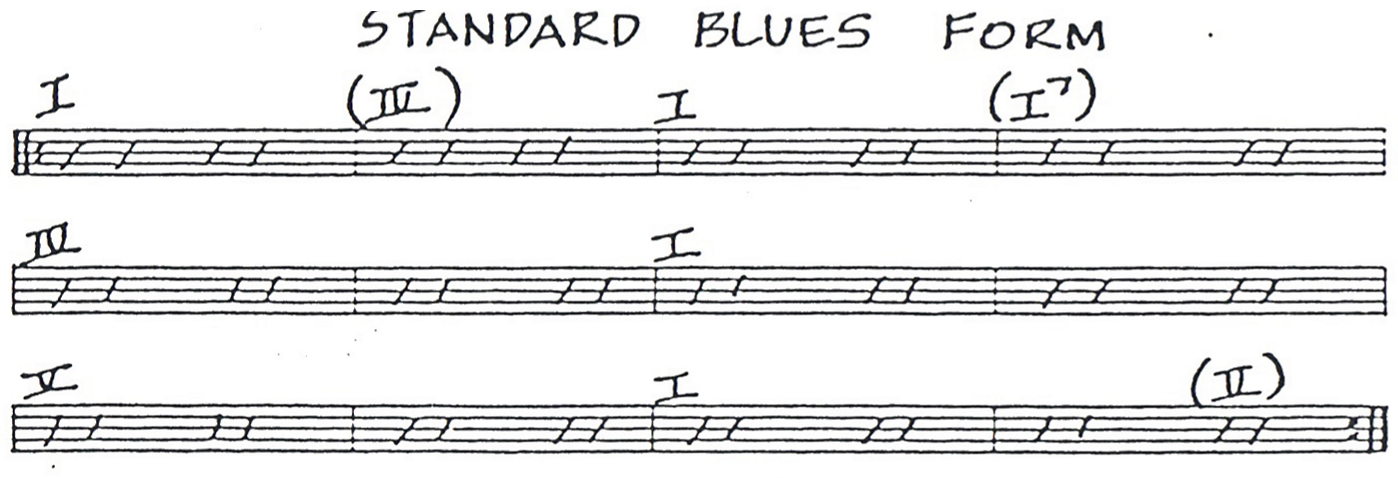
\includegraphics[width=1.0\linewidth]{figures/fig01_standard_blues_form}
\caption{STANDARD BLUES FORM（12小節ブルースの標準和音進行）}
\end{figure}

ローマ数字は和音の根音を表している。各根音に長三和音または長三和音に短三度を積み重ねた短七の和音を各拍子に刻むことが普通である。ブルースには様々な変形があるが、この形式は現在もまだその最も典型的なものとされており、ジャズやロックンロールなど色々なジャンルで用いられているのである。

ここで特に注意すべきことは、七の和音の扱い方である。西洋音楽では長三度に短三度を二つ積み重ねた七の和音は不協和音と見做され、属和音としてしか使われないのだが、ブルースの場合は協和音となっているので、解決する必要はなく、終止音として使うことも普通である。

こうした和音進行の上で行なわれた独唱における唱法が後にジャズの器楽にも取り入れられた。但し、ブルースはもともとアメリカの南部で起こったものであるので、ブルースを全く知らなかった南部以外の奏者のジャズ演奏にはブルースの要素はあまりなかったのである。

\subsubsection{4. アフリカの音楽とジャズ音楽における音色}

ジャズの音色はアフリカの歌唱法や言語と間接的に関係がある。ジャズ奏者の音色は西洋の芸術音楽を勉強して修得した結果ではなく、楽器屋で楽器と一緒に購入したものでもない。ジャズの根本を成すものというのは個性であるので、ジャズの場合は、個性のない音楽家は本当の音楽家ではないのである。

したがって、ジャズ奏者は純粋な音を避け、濁った音色を求めるのである。

\subsubsection{5. アフリカの音楽とジャズ音楽における即興性}

即興というのはジャズの魂でもあれば、その存在理由でもある。ほかにも様々な音楽に関して同じことが言えるので、これは決してジャズにしか見られない性質ではないが、ヨーロッパ系音楽における即興の役割はジャズほど中心的ではない。

複数の奏者が同時に即興を行なうことはアフリカ音楽における重要な原理の一つであり、初期のジャズもこの習慣を引き継いだのである。特にニューオーリンズジャズの場合、多重線的集団即興が特徴である。ところが、「編曲」というものが白人の影響でジャズに取り入れたときにこの集団即興が殆どなくなり、ソリストが一人一人順番に、および問答形式で即興をするようになった。

ジャズにおける即興は、いわゆるフリージャズを除いて、あるソングの和音進行（chord progression）を辿りながら行なわれるものである。その場合、即興をする奏者は、和音が変わるに連れて、適当に自分の弾いている旋律をそれに合わせながら自己表現をするのである。したがってジャズは自己表現の媒体だとよく言われる。

アフリカの伝統音楽やアフロアメリカン音楽と西洋音楽との相違は以上略述したとおりであるが、このアフロアメリカン音楽からジャズが20世紀初期前後に生まれたと推定されている。

\subsection{D. ジャズの黎明期}

\subsubsection{1.　ニューオーリンズ・スタイル}

ジャズの誕生の時期を明瞭に推定するのは困難である。さらに、その誕生に至る詳しい事情は非常に不明瞭である。その出生地はニューオーリンズとなっているわけだが、1900年代から10年代にかけて、同じような傾向がアメリカ各地に現われたのである。ただ、黒人の楽士がやっていた音楽は全てジャズだったとは限らず、地方やその聴衆の社会的地位によって音楽の種類が異なったのである。一般的に言えば、ジャズが演奏された場所というのは紅燈街における酒場や売春宿であった。それ以外にも、ニューオーリンズでは、葬式、共進会等の行事やパーティーでも演奏された。

何故か、ニューオーリンズやその周辺で生まれ育った演奏者の中には、初期のジャズ界に中心的な役割を果たしたものが多かった。したがって、現在まで残っているジャズレコードで最も古いスタイルのものはニューオーリンズジャズと呼ばれる。しかし、その演奏の多くは彼らが1923年にシカゴに移住するまでは録音されなかったので、当初のジャズの実際を知ることは一層難しくなっている。

さて、ニューオーリンズ・スタイルには次の特徴がある。

\begin{gquote}
　1.　旋律：一つの演奏は最初から最後まで殆どが集団即興である。普通はコルネットがその曲の旋律をパラフレーズし、トロンボーンが根音やテノールの対位旋律とグリッサンドを補う。クラリネットが分散和音や装飾音を使って対位旋律を即興する。サクソフォンやヴァイオリンも時々使われる。奏者は声を模倣したような抑揚を使い、ブルーノートを頻繁に使う。多くの奏者がアマチュアであったため、テクニックの水準は比較的低い。\par{}　2.　和声：長音階または短音階を基にした簡単な和音進行。代理和音は用いられない。コードを演奏する楽器、つまりバンジョー、ピアノ、（稀に）ギターなどは、各拍にコードを演奏する。ダブルベース（ピッツィカートで演奏する）やチューバは2/4拍子を弾き、第一拍にコードの主音を
\end{gquote}

\begin{gquote}
強調し、第二拍にその尾音を強調する。\par{}　　3. リズム：ドラムはベースやチューバの２拍子を補強しながら、複雑な行進曲らしいパターンを弾く。後のジャズと比べれば全体のリズムの感じは堅くて、とほとぼ歩く如き調子である。\par{}　　4. 演奏曲目：ほとんどの奏者は楽譜が読めなかったので、作曲もしなかったし、編曲もおそらく演奏する度に変わったと思われる。時々ブレークタイムやストップタイムと呼ばれるテクニックが用いられるが、シカゴジャズほど洗練されていなかったらしい。ブレークタイムやストップタイムというのは、ソリストが即興をしている間にバンドのほかの全員がスタカートのリズムパターンで伴奏を回すということである。レパートリにはヨーロッパの民俗舞曲、ラグタイムの曲、行進曲やポピュラーソングが含まれるが、全体的にはブルースの感じが強い。(Lyons:584頁)　（著者訳）
\end{gquote}

\subsubsection{2. シカゴ・スタイル}

1917年にアメリカのウィルソン大統領が世界大戦に参戦し、ドイツに対して宣戦を布告するとニューオーリンズが軍港となった。そのとき、海軍長官は断固とした態度で、ニューオーリンズの紅燈街、ストーリーヴィルの閉鎖を命令した。

\begin{gquote}
　20年の栄華を秘めたストーリヴィルは、1917年11月に、その歴史の幕を閉じたのであります。あいまい屋、キャバレー、豪華を誇った館は閉ざされ、家具、造作、鏡は競売されました。ウィリー・ピアザの有名な白ピアノは、すでに調子が狂っていましたが、わずか1ドル25セントで落札されました。ストーリーヴィルを追いはらわれたジャズメンたちは、新天地を求めて、ぞくぞく、北上を開始しました。ニューオーリンズジャズは、まるで扇をひろげたように、ミシシッピーの沿岸にひろがっていったのであります。（油井1957:13頁）
\end{gquote}

ニューオーリンズジャズの崩壊をもたらした原因は世界大戦だったのであるが、ジャズバンドをシカゴへ移動させた原因は禁酒法であった。

\begin{gquote}
　...禁酒法は、酒の密造、密輸入、密売をなりわいとし、殺人をものともしない一世の大ボス、犯罪王のアルフォンス・カボネを世に送り出したの
\end{gquote}

\begin{gquote}
であります。\par{}　アル・カポネが禁酒法時代を通じて、たくさんの子分を思いのままに動かし、同業者や邪魔者を殺害し、政治家を買収し、政府の役人、警察首脳部さえも自分の味方として採縦し、組織立った酒の製造販売、シカゴ市周辺に一万軒あるといわれたスピークイージー（秘密酒場）の支配経営にふるった水際だった手腕は、まさに第一級の実業家の才腕と申すべきでしょう。しかも、彼がこの仕事をやり終えた時、年わずかに32歳だったのであります。\par{}　カポネあればこそ、ニューオーリンズを追いたてられたジャズ・ミュージシャンは、状況のわるい禁酒法時代に、シカゴのあらゆる場所で、職を得ることができたのであります。（ibid:14頁）
\end{gquote}

というわけで、禁酒法が1920年に発効されてまもなく、シカゴがジャズの中心地になってしまった。したがって、1920年から禁酒法の解ける1933年までは、ジャズ史上、「シカゴ時代」と呼ばれるのである。

簡単にいえば、シカゴ時代の歴史的な意義の一つは、白人の若いミュージシャンが、黒人たちのジャズを模倣し、白人自らによるジャズを確立したというところにあろう。すでにODJBのような白人ジャズバンドはニューオーリンズにあったが、彼らの演奏はただ黒人の音楽の表面的な要素（主にそのリズム）を取り入れたものであり、即興やブルーノートなど、アフロアメリカン音楽の基本的要素を欠いていたものである。しかし一方では、中西部育ちのクラシックの訓練を受けた白人奏者たちは、南部のブルースなどに関する理解を欠けていながらも、アフロアメリカンたちの音楽の捉え方におけるリズム感、即興法などを見習い、さらに自分たちのクラシック音楽に関する知識を加えてジャズ音楽に和声の面で貢献したのである。

シカゴジャズが次第に野外でなく室内で行なわれるようになるにつれて、巨大な音量が必要でなくなった。その結果、チューバの代りにダブルベース、バンジョーの代りにギターが用いられるようになった。しかし、メロディを担った楽器は依然としてトロンボーン、トランペットとクラリネットであった。

シカゴの白人ジャズバンドが黒人バンドを見習ったにもかかわらず、「白」と「黒」の二つの異なったスタイルが存続したのである。ルイ・アームストロング、キング・オリバー、ジェリーロール・モートンなどニューオーリンズから移ったきた黒人奏者の音楽は、白人のジャズに比べるとリズムがもっと複雑で自由で、ブルースの感じが強かった。一方、ディキシー・ランドとも呼ばれる白人によるシカゴジャズには、ビックス・バイダーベックを含めて中西部からの奏者がいて、彼らはシカゴアンズthe Chicagoansと呼ばれている。彼らはリズム的にラグタイムのように堅い感じがする。白人バンドのレパートリーは主にティンパンアリーの大衆歌曲だが、黒人の方はニューオーリンズのものやブルースが多い。

\subsubsection{3. シンフォニック・ジャズ}

現在、ジャズ史についての一般的な文献ではポール・ホワイトマンの名前はあまり出てこない。ところが1920年代は、ジャズを語る場合、ポール・ホワイトマンをも語らねばならぬ時代であった。

ホワイトマンは主にクラシック音楽界から集めた白人奏者をメンバーとするオーケストラを指揮したが、彼のクラシック的な発想にラグタイムのシンコペーションを取り入れたものは、シンフォニック・ジャズと呼ばれていた。彼は出版社やレコード会社から「ジャズ王」という肩書きを付けられ、誰よりもジャズ音楽を象徴する人物となった。

\begin{gquote}
　ジャズやポピュラー音楽におけるホワイトマンの役割については、今でも盛んに議論されている。一方、極端なジャズ評論家は、彼がビックス・バイダーベック、そしてジャズ全般にとって、有害な影響を与えたと、彼の価値を一切認めようとしないが、大衆マス文化支持者たちは、ホワイトマンはジャズとクラシックの間における偉大な調停者だったという。ポール・ホワイトマンは彼の世代、つまり1920年代における社会の、ある特殊な需要に応じる社会学的現象だったのである...しかし、音楽だけに関していえば、ホワイトマン・オーケストラは称賛に価する業績を多く成し遂げたし、白人黒人両者を含めて多数の奏者がその音楽を尊敬した（場合には嫉んだ）ことは事実である。...ホワイトマンの最も優れた演奏には、ベーシーやエリントンと同様に彼なりに人間らしい、彼独特な響きがする。ただ、ジャズ的発想には基づいていないのである。(Schuller,1968:192頁)
\end{gquote}

（著者訳)

一昔前にジャズ王と名付けられた人物が、今ではジャズ史の文献から採み消されてしまったのは逆説的だが、もしアフロアメリカン音楽から派生したニューオーリンズジャズとシカゴジャズがジャズ音楽の本流であると認める立場を取れば、ポール・ホワイトマンは本当のジャズから外れていたと言わねばなるまい。

\section{第二章　戦前の日本におけるジャズ音楽の定着}

\subsection{A. その歴史的背景}

1970年代になり、あらゆる分野で昭和期を回顧する傾向が顕著になったが、その一環として、日本のジャズへの関心の高まりとともに、ジャズレコードの複刻が盛んに行なわれたり日本におけるジャズ事情についての研究が活発に進められるようになった。詳細な部分はそれらの研究でほぼ明らかにされているので、ここでは簡単にその事実を確認するにとどめておく。

日本におけるジャズの開幕は大正時代とされているが、この時代を理解するために、まずジャズの受容を可能にした、それ以前の文明開化に伴う諸事情を探ることから始めたい。

\subsubsection{1. 軍楽}

徳川幕府三百年の太平の眠りは黒船によって揺り起こされ、日本は新時代の夜明けを迎えた。急速に幕府が勢力を失い、1868年に明治新政府が樹立された。幕末から明治にかけて、諸外国との交流が盛んになるにしたがって、日本における西洋音楽は本格的に発達し始めた。幕府及び各藩においては、すでに鼓隊、鼓笛隊による音楽が演奏されており、殊に紀州藩は喇叭の導入に熱心だった。また、明治2年(1869),薩摩藩は横浜へ30余名の青年を送り、イギリス海軍第10連隊の軍楽長フェントンJohn William Fentonから伝習を受けさせた。それが日本における初の吹奏楽団となり、この軍楽手を中心に明治4年5月、兵部省は海軍軍楽隊の編成を始めた。

\subsubsection{2. 西洋音楽の導入と促進・音楽教育}

富国強兵をめざした明治政府は、そのための人間養成、学校教育に力を入れた。そして廃藩置県の後、明治4年(1871)に文部省を創設し、翌5年に学制を発布した。その時小学校教科の一つとして「楽器に合わせて歌曲を正しく歌い、徳性の涵養情操の陶冶を目的」に「唱歌」という科目が設けられた。一説によると、これは「良い政府には正しい儀式と音楽が必要であるとする儒教の一つの教義」による影響とされている(Waterhouse,1983:287頁)。最初は教師も教材もなく、その他色々難しい問題があったが、唱歌教育の制度は確立し、後にそれを通して西洋音楽が各地で導入されるようになった。

明治12年(1879)、東京音楽学校の前身である音楽取調掛が創立され、以来、全国の音楽教育者養成に大いに貢献した。このように、政府によって奨励された音楽教育は、西洋音楽を一種の教訓として利用したため教育的効果はあったものの、人々の心に浸透するには至らなかった。

堀内敬三は次のように述べている。

\begin{gquote}
　欧米の文化は明治維新以来、決河奔流の勢いで輸入され、欧米の真似をするのが「文明開化」、旧慣を維持するのが「頑固旧弊」と、わけもなく片付けられていたほど世人は欧米に心酔したものであった。しかし音楽だけは勝手がちがった。汽車が走り、電信が架かり、洋燈が点り、洋傘が携えられ、新聞が読まれ、銀座に煉瓦建築が立ち並んでも、洋風音楽は民間には侵入しなかった。（堀内1942：118頁）
\end{gquote}

そして、園部三郎は同じ様な意見を主張する。

\begin{gquote}
　このようにして洋楽の本格的な移植は、上層階級の欧風模倣から始まって、次第に国民の生活の中に浸透していった。しかし、色あざやかに咲き誇る洋花は、透明に磨かれたショーウィンドーの中でこそ、ほこらかに咲きにおうが、その種を別の土壌に移し育てることは決して容易な仕事ではない。\par{}　日本における洋楽は、今日もなおそうであるように、移植の花にすぎなかった。それは上から教えられて覚えられるものであったが、
\end{gquote}

\begin{gquote}
民衆の心にわきおこるものを、その血肉への共感をよびおこすように歌いかなでるものではなかった。（園部1956:6頁）
\end{gquote}

実際に一般民衆にとって西洋音楽を身近なものとしたのは次に述べる職業音楽家たちである。

\subsubsection{3. 洋楽を職業とする音楽家の誕生}

明治20年代陸・海軍軍楽隊退役者が多くなり、その中から洋楽を本職とする者が現われ始めた。したがって、ジャズ音楽が日本に入ってきた当時には、日本人はすでに何十年も前から西洋楽器を用いて仕事をしていたことになる。

その先駆けは加川力氏が率いた「東京市中音楽隊」である。

\begin{gquote}
　「東京市中音楽会」の発生がそれである。これは1886年（明治19年）11月に海軍軍楽隊出身の加川力などが組織した吹奏楽団であって、各方面の要求に応じて手軽に出演演奏をした。この頃吹奏楽なるものは一種のハイカラな流行であって、これを鳴らせば「文明開化」の匂いがしたのである。そのために音楽を聞くという意味でなく、それは商人達の客引き広告宣伝用に使用されるようにもなった。ひいては演奏技術も凋落の方向を辿り、次第に後年の「ジンタ」的性格をおびるに至ったのである。しかしこの市中音楽隊が現今の軽音楽のジャズのごとく、明治初期に一般民衆に洋楽を親しませる大きな役割を果たしたことは認めぬわけにゆかない。（小宮:598-9頁）
\end{gquote}

\begin{gquote}
　欧化された社交の場であった鹿鳴館の饗宴は、華族・士族社会に浸透した。しかし、華族階級ならびに大社会などの園遊会、祝賀会、開場式などでの演奏は、陸・海軍軍楽隊、宮内省雅楽部に申請しても、許可を得ることは容易ではなかった。加川力が、海軍軍楽隊の出身者を主体として、日本に始めての職業演奏家の吹奏楽団を創立したのは、そうした背景があった。\par{}　明治に十一年頃となって、その楽団は「東京市中音楽隊」と名付けられ、職業音楽の発祥となったのである。\par{}　海軍軍楽隊を退役した加川力は、後輩の西村蔵次郎、井上嘉男、
\end{gquote}

\begin{gquote}
蔭ケ原嘉也、平岡啓二郎、古賀貞彦らとともに、平岡の仲介により、花月園経営者の平岡広高と渋沢栄一の出資によって株式会社「東京市中音楽会」の設立をした。そして、洋楽の演奏家を志す若者を募集、二十数名を採用して事務所を芝区愛宕下の薬師寺に置いた。\par{}　（大森:57頁）
\end{gquote}

この「東京市中音楽会」の成功を知った他の軍楽隊退役者は、洋楽の演奏技術を生かす職業演奏家の道が手近にあるのを知り、退役者の多くは職業演奏家の道を進み、「ジンタ」というもの（バンド屋や楽隊屋とも言う）が生まれた。堀内敬三は次のように述べている。

\begin{gquote}
　日清戦役後から日露戦役後にかけて、ちょうど日本の商工業が飛躍的に発展した時代には、広告宣伝用の町回りが盛んに行なわれた。それは市中音楽隊（六七人から十数人）の前後に商品名やら販売店名やら宣伝文句やらを記した幟旗数本づつを人夫が担ぎ、引札配りの人夫が二三人付くという中々大規模なもので、それが毎日幾組も通ったのである。市中音楽隊の広告町回りは全国に行なわれた。「楽隊屋」の数は夥しいものであったに相違ない。\par{}　市中音楽隊―略して「楽隊」と言われた。「ジンタ」という名は大正初期にできたものらしい―は広告の町回りに使われる以外に、曲馬団、パノラマの人寄せに使われ、あるいは売り出し、運動会に使われた。奇術師松旭斎天一の帰朝披露興行大魔術大会が（たぶん昔の明治座で）催された時、その頃妙齢の花形天勝嬢が「胡蝶の舞」のごときものを色電気の光線の中に舞い、嘲哢たるジンタの響きがこれを伴奏したことを私はなつかしく思い起こす。活動写真が神田の錦輝館で時々興行されたときもジンタが伴奏した。浅草の電気館や神田の新戸館が映画の常設館となってからもジンタが伴奏した。すべての「ハイカラ」な催し物にはジンタが参加したのである。\par{}　（堀内1942:255頁）
\end{gquote}

明治41年1月における経済恐慌以降、様々な原因によって町回りのジンタが著しく減少しかつ編成も小さくなり、他の場合においても需要が少なくなった。しかし日露戦争後、映画館が全国に生まれ、ジンタの楽士に新しい稼ぎ場ができた。明治40年代に入ってきたピアノとヴァイオリンも映画館でジンタの吹奏楽に加わるようになった。

\begin{gquote}
　映画館で管弦楽を用いた最初は明治四十三年、浅草のオペラ館で実物応用活動写真ー後の連鎖劇の元祖ー豊香のダンスなどの伴奏に、ヴァイオリン・チェロ・バス・ピアノ・クラリネット・コルネット・トロンボーンから成る合奏を池田辰五郎が楽長となって演奏した時である〔池田辰五郎談〕が、それ以来次第に各館で小管弦楽を用いるようになり、従来の囃子と一緒に和洋合奏などということも始めるようになった。\par{}　...映画館には始めから邦画時代劇の伴奏用として囃子が抱えてあったので管弦楽は忽ちそれと結びついて和洋合奏を始め、これが相当歓迎された。映画館の管弦楽は斯うして段々落ち着いて行った。管弦楽は兎に角こゝで始めて大衆と接したのである。（堀内1942:259頁）
\end{gquote}

しかし、このようにジンタから優秀な奏者が管弦楽団に取られてしまうと、残ったのは腕の鈍い者のみであったので、ますますジンタは凋落していった。

\subsubsection{4. 職業音楽の拡大}

ジンタそのものは衰退して行ったが、その当時、ジンタをきっかけとして、新しい種類の市中音楽隊が誕生し、ジンタのような宣伝用吹奏楽を引き継いだ。つまり、「少年音楽隊」というものである。これは演奏者が自分たちで組んだ独立したものではなく、百貨店の宣伝道具として作られたものである。三越の日本橋本店と大阪支店を始めとして五つの百貨店が明治末期から大正時代にかけて洋楽演奏者を養成し、日本の職業音楽界において多くの人材を供給したのである。

\begin{gquote}
　大正初年頃（1912年）、「今日は帝劇、明日は三越」という言葉がはやった。その日本橋三越が明治42年（1909年）2月16日、店の宣伝のために少年音楽隊を作った。四月の第一回児童博覧会（現・同店の敷地）に早くもライト・ブルーに金ボタンのかわいい姿で現わ
\end{gquote}

\begin{gquote}
れ人気を集めた。（内田32頁）
\end{gquote}

後に名古屋の松坂屋(1911)、大阪の高島屋(1923)、大阪の出雲屋(1923)

で少年楽隊が結成されたが、1925年には大震災による不況に対する経営の緊縮策として三越両店と高島屋の楽隊が解散された。1927年、東京練馬区の豊島園が解散した三越から久松鉱太郎を指揮者として雇い、豊島園少年楽隊を結成し1929年まで続けた。

その中で最も寿命が長かったのは松坂屋で、1932年名古屋交響楽団、1940年中央交響楽団、1941年東京に移り東京交響楽団と改称を続け、1945年の大空襲ですべてを焼き解散した。（内田32-37頁）

さらに大正期に於ては西洋音楽を需要とする娯楽産業（ダンスホール、新劇、映画館、浅草オペラ、宝塚レビュー、など）が次第に発展し、西洋音楽の職場は拡大していく一方であった。そのため、大衆はようやく洋楽器の音や洋楽的な旋律や和声など、調性音楽に多少慣れて行ったのである。

一方、1912年から商船会社の北米航路が船に楽士を乗船させ始めた。

これは約20日間に渡る長い航海の退屈を慰めるために、食事時の音楽、社交ダンスの音楽を演奏するものであった。この船のバンドの乗船は1912年から太平洋戦争が勃発する寸前の1941年8月まで29年間継続され、その航路からおびただしいアメリカンポピュラーソングが国内に流入した。その船のバンドのメンバーがジャズ演奏の技術を国内に持ち込んだのであった。その技術を国内のバンド屋、デパート音楽隊などが修得し、広めていった。（内田晃一談）（大森:98頁参照）

日本へのジャズ音楽伝来におけるもう一つの要因はフィリピン人演奏家である。ジャズ音楽においてフィリピン人が日本人より進んでいたのは当然である。1898年以前スペイン領であったフィリピン諸島はそれ以降アメリカが占領したので、アジアのどこよりもアメリカの大衆文化が支配的で特にアメリカの音楽は隆盛を極めた。しかも1920年代から30年代にかけての間はフィリピンにおける娯楽の黄金時代だったのである。

日本のジャズにおけるフィリピン人の影響について、大森盛太郎は次のように書いている。

当時、【1920年代】マニラを起点に運航をしていたバンクーバー及び北米航路があった。エンプレス商船会社系の「エンプレス・オブ・カナダ」「ジャパン」「ロシア」が運航していた。それに日本の「大洋丸」「これや丸」などが加わり、その五船にフィリピン演奏家が乗船していた。寄港する各港でもジャズ音楽が発展、東洋の主要都市の各地にジャズ音楽の進路を開いていった。

フィリピンのマニラには、マニラ・ホテル、およびサンタアナならびにマイバエの両キャバレーがあり、香港には香港ホテル、リパルス・ホテル、ピーク・ホテル。上海にはサヴォイ・ホテル、キャセイ・ホテル。神戸にはオリエンタル・ホテル、横浜には、横浜グランド・ホテルなどがジャズ音楽の基点となった。それらのホテルで...米国人系、フィリピン系のジャズ演奏家が演奏していた。

そしてフィリピン演奏家が日本で多く働いていた。

その理由の第一には、大正八年ごろすでに神戸オリエンタルホテルでP・アントニオ、ベベ・マテアスの両楽長らの楽団がサロン音楽、ダンス音楽の演奏をしており、大正十年には、ホセ・アルカンタル楽長〈ドラム〉、．．．など引き続いて、毎土曜日の夜、ダンス音楽を演奏していた。また、米国ジャズ音楽の流行が、時の流れにのって東洋にも浸透し、日本の職業音楽界に大きな影響をもたらしたのである。

第二には、神戸に在住していたフィリピン演奏家の多くが日本婦人と国際結婚をして定住していた。

第三には、オリエンタルホテルで演奏するフィリピン楽団が大阪のカフェーおよびダンスホールへも進出し、ジャズ音楽を演奏していた。

第四には、日本の若い演奏家の中には新しい波のジャズ音楽に魅力をもち、その演奏に対して志向動向を示していたということである。

このように米国音楽文化の一端たるジャズ音楽が、日本に流布する背景には、商機に強い大阪のカフェー界、それにダンスホールの新設などによってジャズ音楽が求められるようになっていたからでもある。

こうした要因のもとに、ジャズ音楽が神戸から大阪へと流れ、職業音楽としても昭和期には「本格的ジャズ」の成熟期に入るのである。（大森:144-45頁）

\subsection{B．戦前の日本におけるジャズ・その音楽の分析}

日本でジャズを始めて演奏しだしたのは、以上述べた、すでに洋楽を職業としていた楽士たちである。さて、これらの楽士が演奏したジャズ音楽は、実際にどのようなものだったのであろうか。その主なる人物の詳細については、最近数多くの研究の中で盛んに論じられているが、戦前の日本のジャズ音楽そのものにおける楽曲分析は殆ど行なわれていないのである。したがって、いくつかの代表的な録音を参考にしながら、日本のジャズ音楽の特徴を説明したいと思う。

\subsubsection{1．「ジャズソング」以前のジャズ}

日本で最初にジャズバンドと呼ばれるものが現われたのは1921年である。

\begin{gquote}
　　...浅草へ進出した松竹は、（大正）10年6月17日から帝国館でジャズバンドを演奏、同時に金春館でもジャズをはじめている。（倉田1979:250頁）
\end{gquote}

しかし、当時はジャズレコードというものはなかった。

\begin{gquote}
　　ジャズと銘打ったレコードが、突然目につきだした。活動写真館では、すでに大正10年から演奏されているが、レコードとしては14年11月から。各社とも専属の楽団をかかえ、今まで聞き慣れなかった片仮名の名称を付ける。グループごとに、どのような曲を演じているのか眺めてみよう。
\end{gquote}

\begin{listblock}
Carl's Show Jazz Band:(日蓄)\\
14.11 Saint Louis Blues Medley\\
14.12 Hong Kong Dream Girl That's my girl\\
15.1 Copenhagen Hard Hearted Hanna\\
Philippine Jazz Band\\
14.11 I want to be Happy Honolulu\\
15.2 Oriental Dance, Tee Teen on Me\\
Orchestra Rhapsody\\
14.11 Serenade Blues/Three o'clock in the morning\\
Mandolin Inn Orchestra\\
14.11 Foot Warmer/Some of these days\\
15.1 All Alone (Waltz)/Wonderful one (waltz)\\
大阪松竹座管弦楽団（オリエント）\\
15.7 アフガニスタン舞踏曲、チチナ\\
15.8 猫おどる、赤ちゃん\\
（ibid:296-7頁）
\end{listblock}

当時のレコード会社の月報には「ジャズ」または「ジャヅ」という項目があり、そこに載っているのは上の列記と同じように外国の曲、主にティンパンアリー曲がほとんどである。しかし、これらは日本における最初のジャズレコードと言ってよいのであろうか。実は、いわゆるジャズバンドによって、同じような曲は前から録音されて発売されていたが、今度は名称が変わっただけである。

ここで注意しなければならないのは、フィリピン人のジャズバンドが目立った点ある。「Philippine Jazz Band」はもちろん文字どおりであるが、「Carl's Show Jazz Band」もフィリピン人によるバンドであった。

『不滅日本ジャズポピュラー史』という三枚組レコードには、日本人もフィリピン人も含めて1920年代前半におけるジャズレコードの復刻版が入っている。日本人の波多野オーケストラや天洋丸管弦楽団の演奏を、フィリピン人のカールトン・ジャズ・バンドや日本人とフィリピン人両方が入っているニットー・ジャズ・バンド（瀬川昌久談）の演奏と比較してみると、フィリピン人が参加しているバンドの方が進んでいるのが分かる。

船から上陸した波多野オーケストラの《オリエンタル・ダンス》(1923吹き込み)は、管絃楽器に太鼓とバンジョーを加えたものであるが、全体のリズムは単純で堅く、シンコペーションやリズム単位の均等化はない。天洋丸管弦楽団の《ウイズ・ザ・カミング・オブ・トモロー》(1923吹き込み)はスーザの曲にも思える吹奏楽器による行進曲である。

これらに対して、ニットー・ジャズ・バンドの《ワラー・ワラー》

\begin{gquote}
（1925吹き込み）とカールトン・ジャズ・バンドの《フー》（1927吹き込み）は、一部では歌が入っており、アメリカ人によるものと思えるほど発音がうまい。メロディの楽器はシンコペートされたリズムで即興演奏し、一部では楽団即興があって、シカゴジャズと類似している。また、バンジョーは各拍にコードを鳴らすが、弱拍（4/4の第2と第4拍）を強調しているのでスイングの感じがもたらされる。常にメロディが聞こえるが、楽譜どおりでなく、即興的に変奏されているようである。また歌手やコーラスが歌っている部分より楽器のみの部分が長い。
\end{gquote}

1925年頃のレコードでは、このようなジャズらしいものはまだ比較的珍しいが、西洋楽器を伴奏に歌うというものはそのあたりから始まった。それ以前の西洋音楽の録音はすべて器楽であって、声楽といえば三味線が伴奏をしているものであった。西洋器楽に歌が加わり始まると次第に歌が中心となって行った。

\subsubsection{2．ジャズソングの登場以降のジャズと流行歌}

1928年までのレコードはすべて喇叭吹き込みであった。それ以降電気吹き込みとなり、音質が著しく改良されたのである。同時に、新しくできたビクターとコロムビヤ両会社はそれまでのレコード会社と違って積極的な姿勢を取り、歌をはやらせようとしたのである。そうなると、レコード会社が映画会社と連携して曲をはやらせることが頻繁に行なわれ、レコード一種当たりの最大売上が数千枚から数十万枚へと上昇した（倉田1979:333-4頁）。こうした背景で最も売れたのは西洋楽器を伴奏に使った洋風の歌であり、それは「ジャズソング」と呼ばれるようになった。ジャズソングにはティンパンアリーの曲に和訳した歌詞をつけたものと日本人が作曲・作詞したものの二種類がある。

初めて外国の流行歌を日本語に訳した堀内敬三は、1933年の論文で初期のジャズソングとその急速な進歩について次のように語っている。

\begin{gquote}
大正十五年の十月に私が放送局へ入ってから、新交響楽団の楽員中からジャズのすきな者を集めて「JOAKジャズバンド」というもの
\end{gquote}

\begin{gquote}
を作って度々放送した。これもあまりうまくなかったが、どうせ放送すべきものなら外人のよりは日本人のジャズを放送した方が気が利いていると思ったのである。少なくとも、JOAKジャズバンドの連中は譜が読めたから非音楽的な演奏をやらないという安心があった。そのうちにジャズに歌をいれる必要を感じてきた。外国のジャズバンドでは楽手が歌うが日本のジャズバンドの人は歌わないから、天野喜久代、二村定一両君にたのんで昭和三年の二月に「バレンシア」「アラビアの歌」などを私の邦訳で歌ってもらい、以後これを続けた。日本語のジャズソングはこれから始まったのである。日本人がジャズソングを好むものならば、この方面にも日本人の作曲が出なければならないと考えた。先ず隗より始めよというので、フォックストロットの「黒い瞳」タンゴの「旅人の歌」などを作り自分でジャズバンド用に編曲して、偶然にもこの方面の先駆をしてしまった。しかし私はジャズの選手たる資格はないのである。第一私は踊れないし、ダンスがすきでもない。純粋に音楽上の興味からジャズに干与しただけだから、この方面に優秀な楽人が現われて、芸術的なジャズ音楽を大衆に供給するようになると、早速ジャズの実際方面から退去して鑑賞者の一人となった。現に日本人のジャズバンドは草創時代と比較にならない程上手になっているし音楽的にもなっている。作曲者にも紙恭輔君の指揮するPCL管弦団の如きは、高級なジャズ演奏団体として優秀なものである。作曲者にも紙君、松竹の田代君、ビクターの佐々木君などのような俊才も出ている。歌い手も川畑文子君、淡谷のり子君、其他雲の如くである。今回報知新聞社主催のジャズ祭に対して私は僅か数年の昔を回顧して隔世の感に打たれる。（堀内1934:78-80頁）
\end{gquote}

この論文から、「JOAKジャズバンド」が「度々放送した」ジャズとは、まず、楽譜どおり演奏された器楽であったことが分かる。つまり即興はあまりなかった。ここで日本語によるジャズソングの初放送は1928年2月とされている。実際にジャズソングが流行するのはその翌年の5月《東京行進曲》が発売されてからである。それ以降、日本のジャズは流行歌と密接に発展して行ったのである。

現在《東京行進曲》を聞くと一体何がジャズ的なのであろうかと思うかも知れない。即興も、スイングのリズムも、ブルーノートも何もないので、理由はその歌詞にジャズという言葉が出てくるからだけと思うかも知れない。日本的にさえ聞こえるかも知れない。ジャズ的ではないが洋風だからジャズソングといわれるのである。その当時、洋楽器による洋風の曲に日本語の歌詞を付けたものを初めて聞いた大衆にとっては、恐らく驚天動地のことだったはずである。

しかし、どこが洋風なのであろうか。楽譜を眺めてみよう。

\begin{figure}[H]
\centering
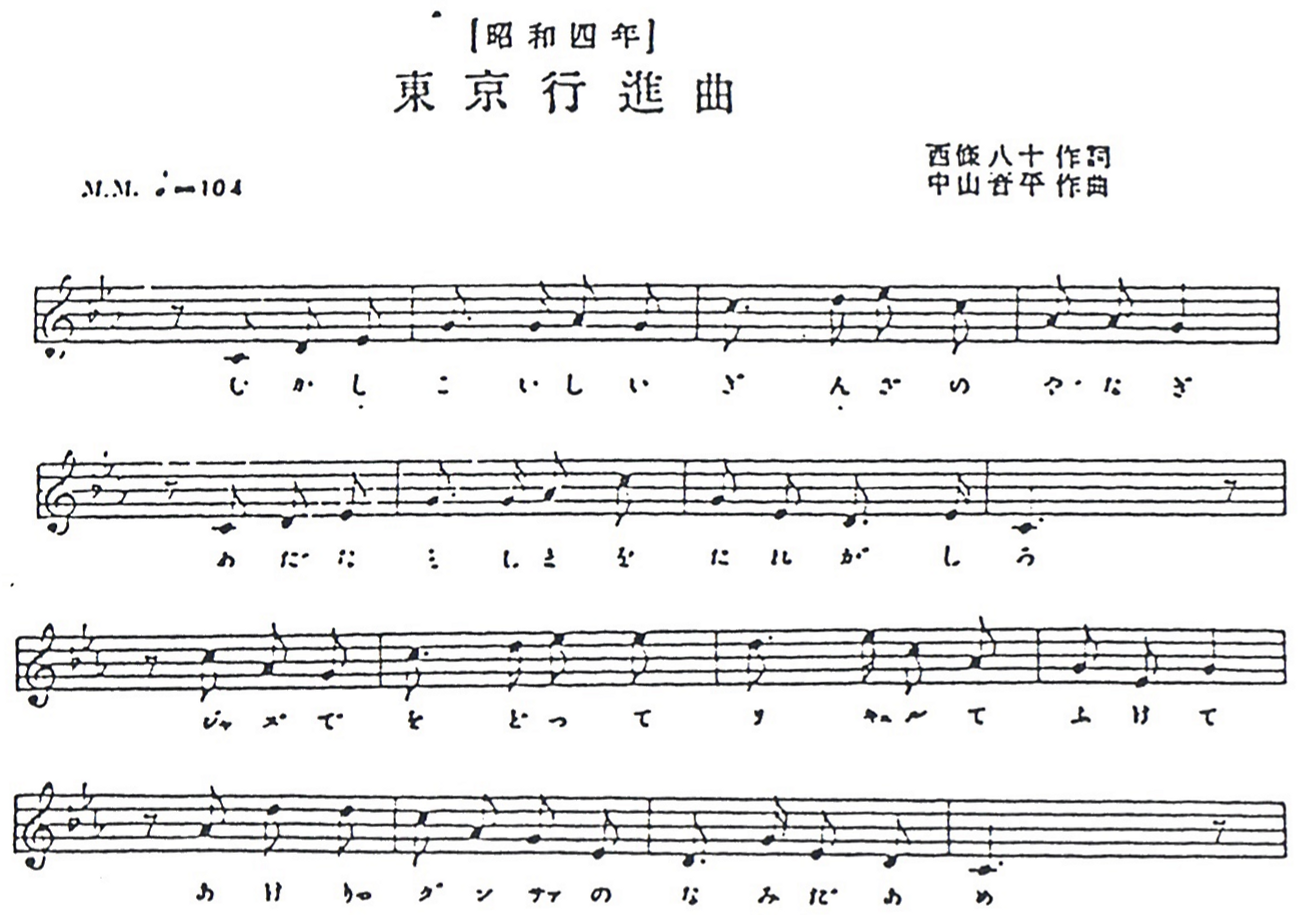
\includegraphics[width=1.0\linewidth]{figures/fig02_tokyo_koshinkyoku}
\caption{《東京行進曲》（昭和四年）　西條八十作詞・中山晋平作曲}
\end{figure}

まず、江戸俗曲の名残に思われるのは、近世小唄調と呼ばれる歌詞における音節のパターン（7・7・7・5）である。ヨナ抜き短音階は、実は明治以降の和洋折衷である。しかし明確に西洋的な要素が四つある。

\subsubsection{1．形式における対称性（シンメトリー）}

江戸俗曲は、都々逸にしろ、大津絵節にしろ、非対称的な形式がほとんどである。一方、西洋音楽では、讃美歌、吹奏楽、ティンパンアリーの曲などにおいては対称性は当たり前のような根本原理である。

西洋音楽を重んじた中山晋平は、対称的な形式を好んで、多くの対称的な曲を作った。12小節の《カチューシャの歌》には三つの対称的なフレーズがある。また、《ゴンドラの歌》は6/8拍子で、《東京行進曲》と同じように4つのフレーズから成り立ち、各フレーズに4小節がある。

\subsubsection{2. 調性音楽の特徴（和声や和声構造における終止形の使い方など）}

調性音楽の場合、最も単純な和音進行は主和音－属和音－主和音である。なぜなら、ある曲は必ず特定の「調」でなければならないし、その調を決めるのは終止形だからである。そして最も簡単な終止形は上記のものである。

日本人が初めて歌に和声をつけたときは主音上の三和音であったが、次に用いられた和音は属和音であった。そのときに属和音の緊張性が主音の安定性へと解決され、ゆえに調性がもたらされたのである。後の流行歌において調性というものが根付き、現在の民謡でも、演歌でも、ポップスでも、すべては「何々調だ」ということが言える。

\subsubsection{3. 洋楽器編成}

すでに述べたように、日本語の歌に洋楽器の伴奏を付けたものはまだ比較的新しかった。一般民衆は、調性や形式などの新しい音楽要素よりも「ジャズバンド」のハイカラな音色を意識していた。

\subsubsection{4. 西洋的な発声法}

唱歌教育の結果であろうが、初期の洋風流行歌にはいわゆる「ベルカント」で歌う傾向が強かった（演歌や民謡における難しいこぶしは戦後数年まで見られなかった）。これは、アフロアメリカン音楽における発声法はまだ伝わっていなかったということを証明している。西洋の歌における様々な発声法は皆同じものと思われたようである。

対称的な形式、調性、洋楽器編成、西洋的な発声法。この四つの特徴は以降のほとんどの流行歌に共通している。本来のジャズからの影響よりも西洋音楽教育の影響が圧倒的である。しかしこれがジャズとされてしまった。

1931年、松竹映画が『マダムと女房』という、日本における初の本格的トーキー映画を計画し、その中で近代を描写しようとした。トーキー映画だから音声をうまく利用しなければならないということであった。したがって、自動車や飛行機の音、鰹節を削る音、目覚まし時計の音、紙を千切る音などが入っている。そして、やはりジャズバンドの騒音をも入れなければならなかったのである。そのための主題歌を委嘱し、帝国館ヂャズバンドに演奏させた。映画では「Mammy Jazz Band」となっている。作曲は高階哲夫、作詞はサトウ・ハチロウで、曲名は《スピード時代》である。

\begin{figure}[H]
\centering
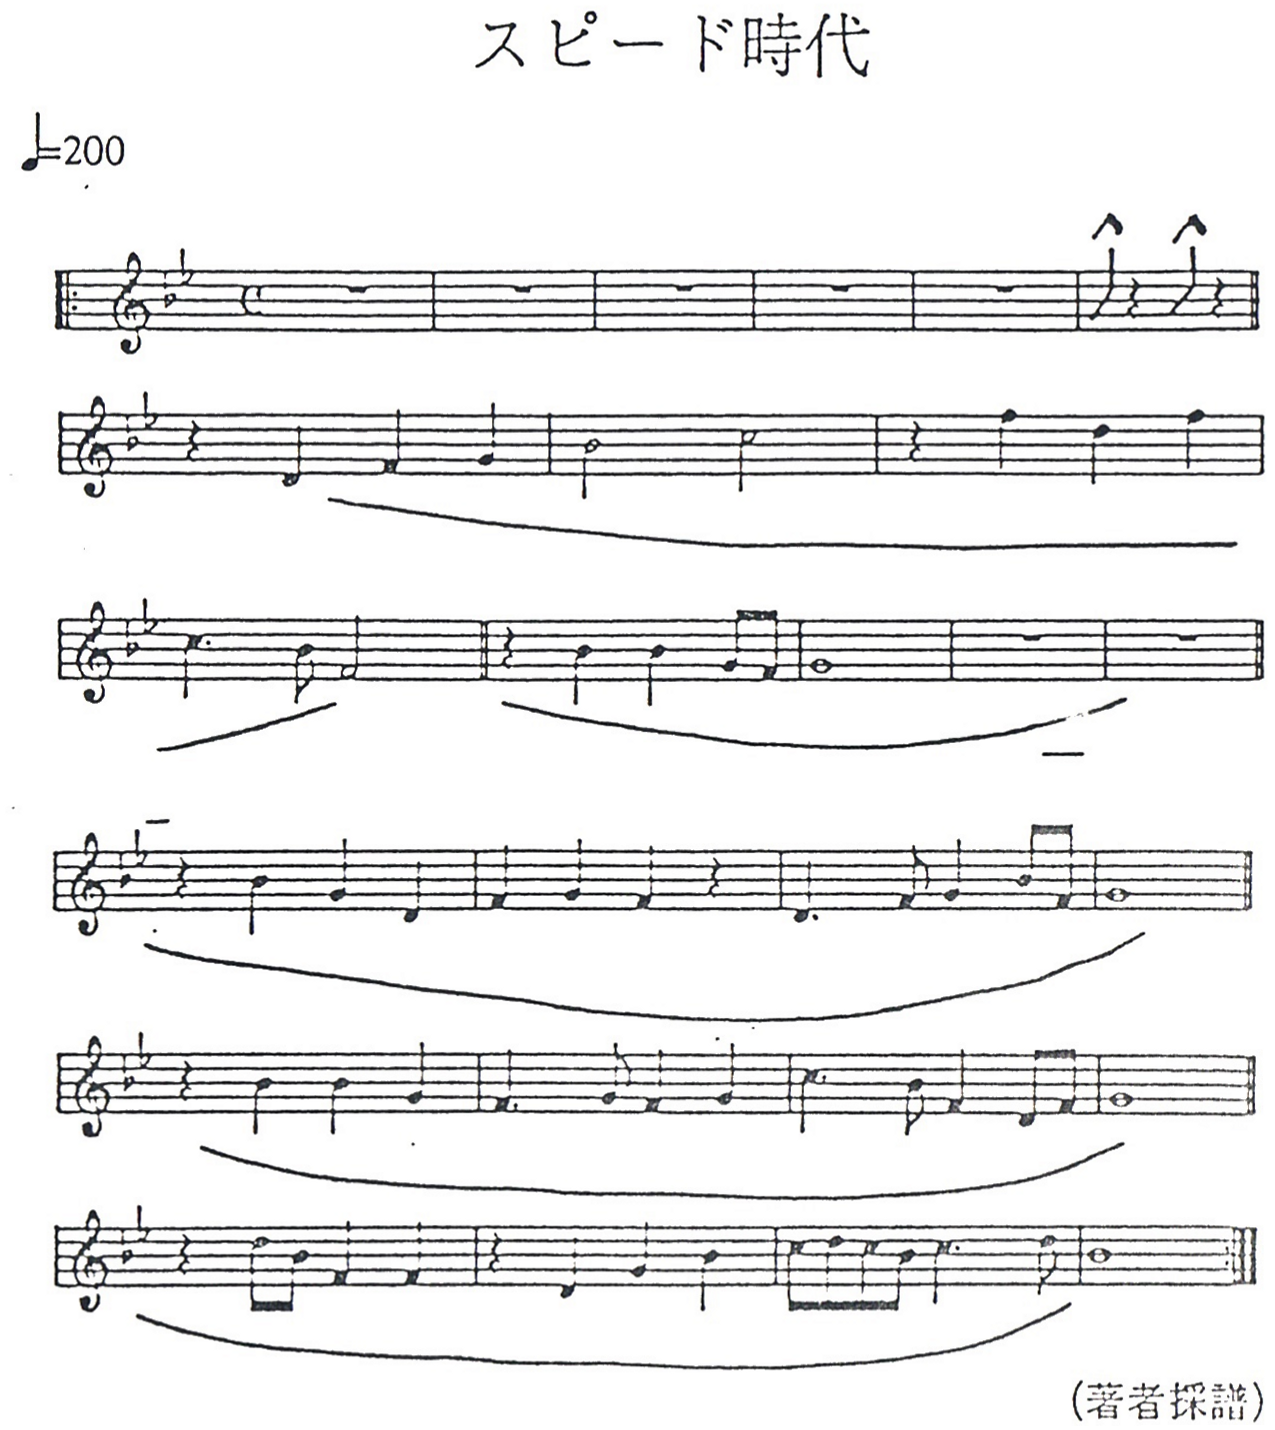
\includegraphics[width=0.92\linewidth]{figures/fig03_speed_jidai}
\caption{《スピード時代》　高階哲夫作曲・サトウハチロウ作詞（著者採譜）}
\end{figure}

この曲と演奏は、けっして当時として優れたものとは言えないが、最初のトーキーで使われたジャズソングとして、ならびに当時の映画館ジャズバンドを代表するものとしては意義がある。

楽器編成はバンジョー、トロンボーン、トランペット、サクソホーン、ドラム、ウッドブロック、ピアノと木琴である。リズムにおいては強拍が強調されているし、シンコペーションやポリリズムもないのでスイングしていない堅いリズムである。バンドの全員は皆それぞれ出鱈目に即興で弾いているので不調和的で騒がしいものである。歌手の市村美津子はやはりベルカントで歌っている。

この形式は6・4・4・4・4・4（小節の数）で構成されており、それが何回か反復されている。歌が入っている部分は、フレーズは皆4小節ずつである。低音を出す楽器がないためコードの主音がはっきりしない。5小節目にはFの長三和音、6小節目にB♭の長三和音が聞こえ、旋律の最後のフレーズもB♭で終止するので調はB♭長調だと言えよう。しかし、その間の部分は終止形がないので和音進行は曖昧であまり和声の緊張と解決を感じない。

このような弱い調性の楽曲は主音をはっきりさせるためにリズム的終止形を使っている。6小節目のリズムはそうである。つまり調性音楽に慣れていなかった作曲家のテクニックである。

\subsubsection{3. ジャズ的流行歌の登場}

一般民衆にとってはジャズの代表的なものは《東京行進曲》や《スピード時代》のようなものだったかも知れない。しかし一方、演奏者の一部では本来のジャズに興味を持った者がいて、彼らは熱心にアメリカの本格的なジャズレコードを勉強していた。

南里文雄はその一人である。彼は1929年に上海に渡り、7ケ月そこに在留した間に、かつてルイ・アームストロングと一緒に活躍していた偉大なピアニストTeddy Weatherfordに師事をした。帰国の際に自分のジャズバンドを組み、本格的なジャズ演奏をした以外にも、他の多くの演奏者、歌手などのレコードにも加わった。

1934年にはディックミネは新しくできたテイチクにはいり、彼の最初のレコード《ダイナ》の録音に南里と彼のバンド「ホットペッパーズ」がその伴奏をした。このレコードでは、それまでのジャズソングと違って、長いイントロがあって、それから歌があって、最後に再び器楽の部分がある。このレコードが著しく流行し、一世を風靡したのである。以後各レコード会社は、《ダイナ》の恩恵に浴そうとして、それぞれの《ダイナ》を発売した。

\begin{gquote}
　「こうした"ダイナ旋風"は、日本のジャズ感覚を大幅に修正させたようだ。かつて売れなかったジャズ・レコードは、ダイナによって過去のイメージを払拭したのである。」（倉田1979: 416頁）
\end{gquote}

ここで、南里文雄が演奏したソロを取り上げてみよう。

\begin{figure}[H]
\centering
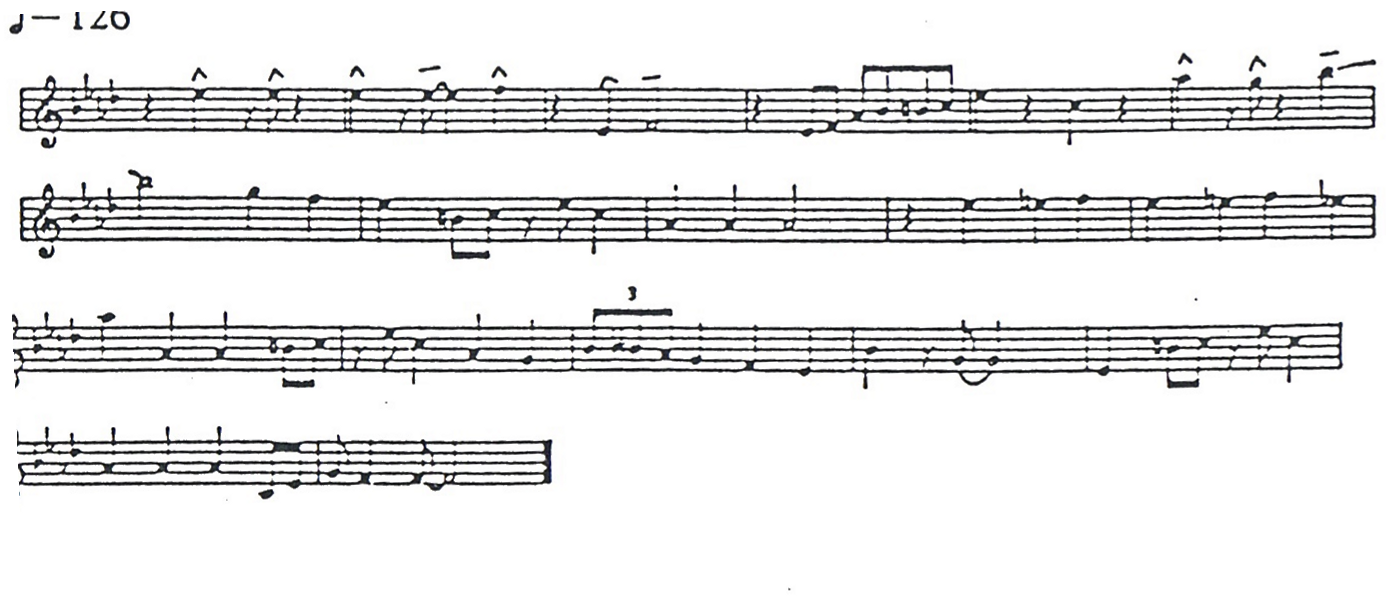
\includegraphics[width=1.0\linewidth]{figures/fig04_dinah_solo}
\caption{南里文雄の《ダイナ》ソロ採譜　♩=126（著者採譜）}
\end{figure}

\begin{verseblock}
和音進行\\
Eb,Eb,Ab,Ab,Ab,Ab,\\
Eb,Eb,Ab,Ab,Ab,\\
Ab,Ab,Ab,Eb,Eb,\\
Ab,Ab
\end{verseblock}

このソロは短いが、非常に優れたものである。ここまでのテンポは♩＝126であるが、南里のソロの冒頭にテンポが倍になっている。

このソロにおける素晴らしい点は3つある。第一はそのリズム感におけるスイングである。各音は的確に演奏されているが、前向きの方向性が感じられる。リズムは非常にシンコペートされたし、弱拍と強拍も均等化されている。

第二は南里の優れた和声感である。この部分は二つの和音しかないので、それに合わせて即興演奏で前向きの方向性を感じさせることは難しいが、南里はその次に続く和音進行に先立って先行音を弾いている。例えば、6小節目のGとB♭は15小節目のE♭長三和音（属和音）を先取りしている。また同じように14小節目のB♭・G・E♭は15小節目のE♭長三和音を先取りしている。8小節目のC・E♭・Cは9小節目のA♭長三和音を先取りしているし、16小節目と17小節目も同じである。

第三は彼の優れた音色である。各音における音高は明確であるが、各音に抑揚を付けたり、ビブラトを長い音に付けたりしている。ルイアームストロングを連想させるような音である。

1936年から「何々ブルーズ」（または「何々ブルース」）という曲名が目立ってくる。その第一号は谷口又士（トロンボーン奏者）の作曲した《想い出のブルース》であるが、後に《雨のブルース》《別れのブルーズ》《広東のブルース》《想い出のブルーズ》（服部良一作曲）《上海ブルース》《熱海ブルース》《夕空ブルース》《東京ブルース》（二つ）《伊豆ブルース》《佐波ブルース》《桜ブルース》などなどの洪水が溢れる。（辻1985参照）

これらのいずれもは歌詞は憂鬱で旋律は短調で形式はいくつかの四小節フレーズから成り立つ。しかし、本来のブルーズと違って、三つの四小節フレーズから成り立つものはないし、曖昧な調性も、旋律におけるブルーノートも見られない。

服部良一の《別れのブルーズ》はその代表的なものの一つである。

\begin{figure}[H]
\centering
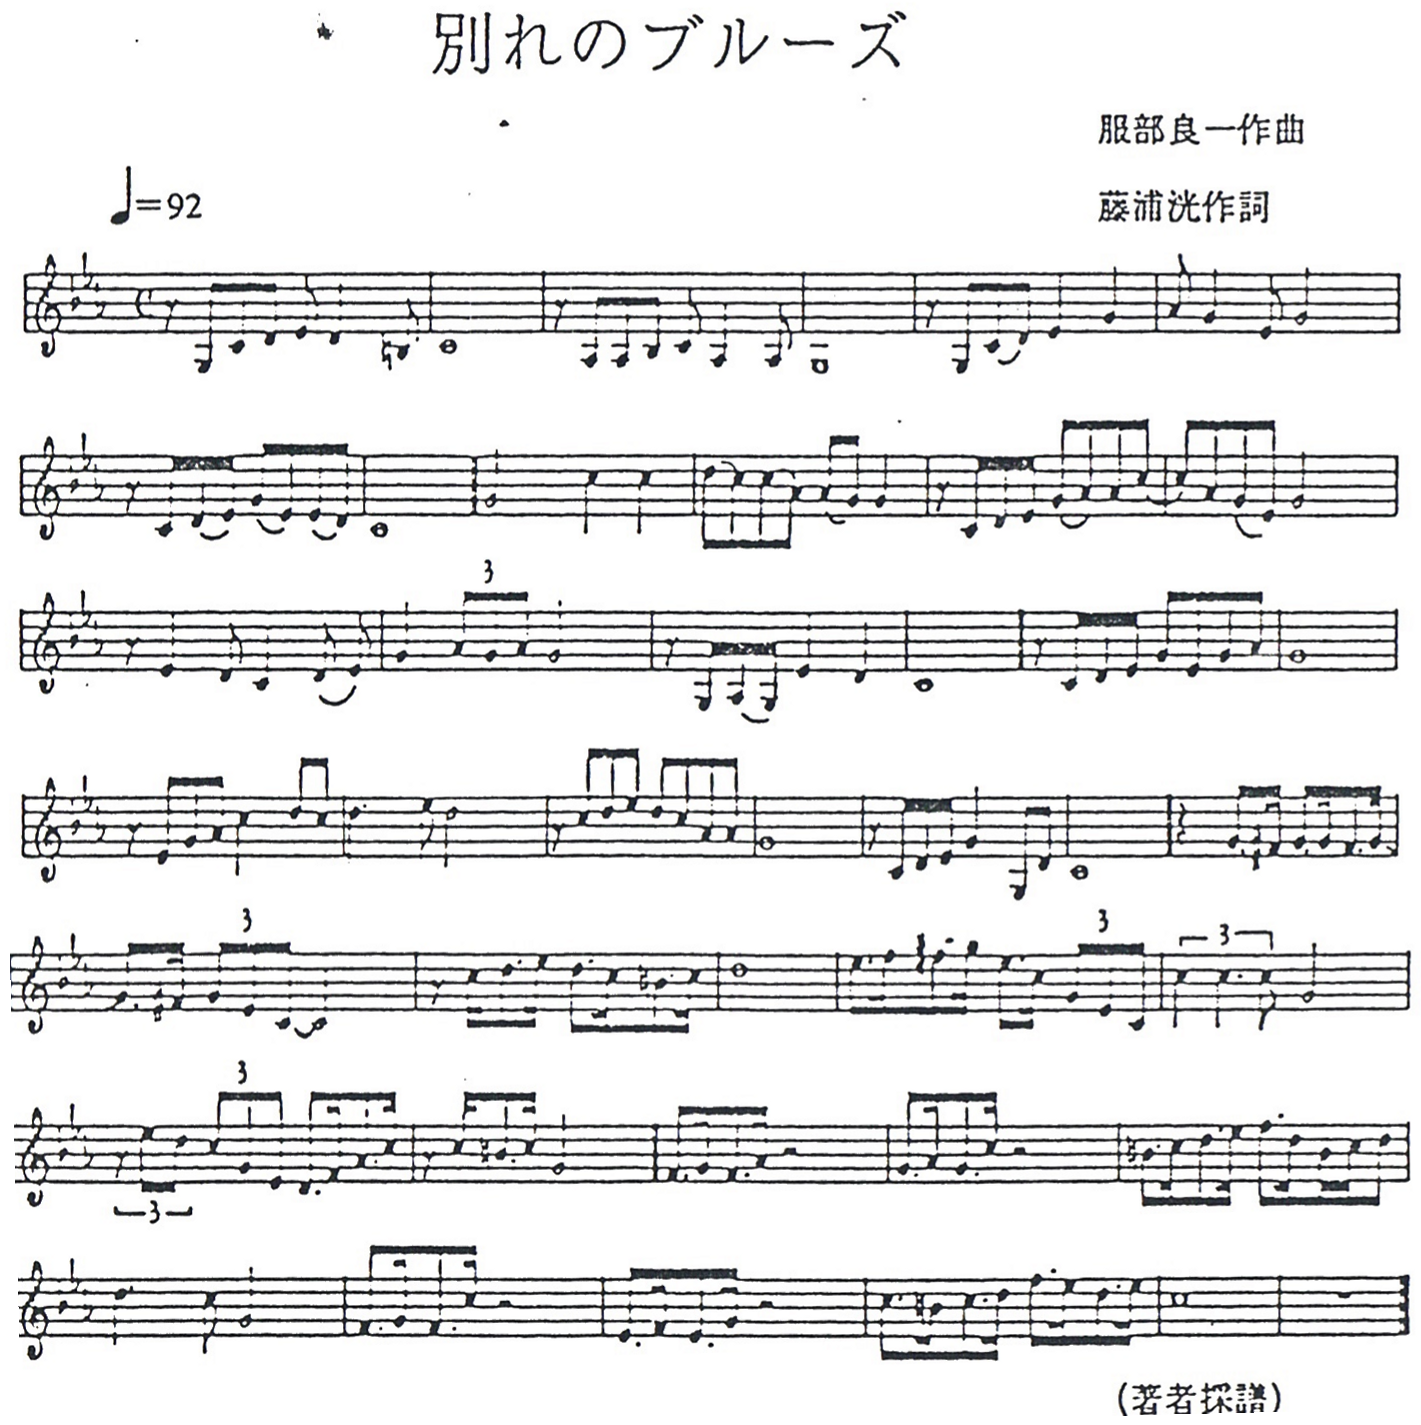
\includegraphics[width=0.78\linewidth]{figures/fig05_wakare_no_blues}
\caption{《別れのブルーズ》　服部良一作曲・藤浦洸作詞（著者採譜）}
\end{figure}

\begin{verseblock}
和音進行\\
（歌）Cm,Cm,Fm,Cm,\\
Cm,Cm,A♭7 G7,Cm\\
Cm,Fm Cm,Cm,Cm
\end{verseblock}

\begin{verseblock}
Cm,Cm,G7,Cm\\
Cm,Cm,Cm,G7,\\
Cm Fm, Cm,Cm G7,Cm\\
（トランペット間奏）\\
Cm,Cm,Fm,G7,\\
Cm,Cm,Cm Fm,Cm,\\
Fm,Cm,G7,G7 Cm\\
Fm,Cm,Ab7 G7, Cm,(Cm)
\end{verseblock}

\begin{verseblock}
歌詞\\[0.9em]
窓を開ければ港が見える\\
メリケン波止場の灯が見える\\[0.9em]
夜風汐風恋風乗せて\\
今日の出船は何処へ行く\\[0.9em]
むせぶ心よはかない恋よ\\
踊るブルーズのせつなさよ
\end{verseblock}

レコードレーベルでは「ブルース」となっているが、歌詞カードではタイトルも歌詞の中でも「ブルーズ」となっている。

形式は対称的で、三つの長い8小節フレーズがあって、それぞれの長いフレーズは四つの2小節ずつの短いフレーズから成り立っている。和音進行はフレーズ構成にしたがって整理されていて、長いフレーズの最後に属七和音から主和音の終止形がある。そのため、調性がはっきり感じられる。

間奏の前半はトランペット・ソロ（即興演奏であるかどうかは不明瞭である）となり、後半はオーケストラとのトゥッティである。間奏の最後に余分の1小節が付け加えられている。

日本のブルーズは何故こうなっているのであろう。これは明らかに序論で説明したのと異なるものである。実は、服部良一の自叙伝にその理由を明らかにする糸口がある。

服部は、ジャズの本物はハンディ W.C. Handyの《Saint Louis Blues》だと信じていたのである。ハンディの書いた『ブルーズ』という本をも読んでいた。日本にまで普及してきたブルーズの中で《Saint Louis Blues》が最も早かったからであろう。（服部1982:139-148頁）

《Saint Louis Blues》の構成を取り上げてみよう。

\begin{gquote}
和音進行‖F,B♭,F,FB♭,B♭,F,F,C7,C7,F,F‖‖Fm,Fm,C7,C7,C7,C7,Fm,FmFm,Fm,C7,C7,C7,C7,Fm,Fm‖
\end{gquote}

最初の12小節は明らかに典型的なブルーズ形式である。和音進行では長三和音となっているので、その上にブルーノートを歌えば曖昧な長調でもなければ短調でもない調性がもたらされる。ところが、後半は短調であり、しかも16小節の形式である。服部が作曲したブルーズはハンディの非ブルーズ的なブルーズに由来しているのが明確である。

これについては異説を取り上げてみよう。

\begin{gquote}
　都々逸の歌詞が七七七五であるというのと同じように、ブルーズの最も単純な定義は、12小節で歌詞は三行、歌詞内容はAABというものだ。藤浦洸が小節の数や長さを合わせるために参考したのは「セントルイス・ブルーズ」だろうから、両者を合わせてみると確かに対応するのである。
\end{gquote}

\begin{verseblock}
I hate to see that evening sun go down.\\
窓を開ければ、港が見える\\
I hate to see that evening sun go down.\\
メリケン波止場の灯が見える\\
'Cause my baby, he's gone left this town.\\
夜風汐風恋風のせて　今日の出船は何処へ行く
\end{verseblock}

\begin{gquote}
対応である。訳しているわけじゃない。「セントルイス・ブルース」の方は、AABの三行、それに沿って「別れのブルース」もAA'B型、形式だけではなく内容も、時刻の夕刻、恋人が船で去るだから気持ちもブルー（憂鬱）だと踏襲していると理解してもいい。ただし歌詞内容面に関しては、ブルースも演歌も失恋は常套句だから似てしまうのはあたりまえだが、日本ブルース演歌成立の初心で藤浦洸が当時世界中でいちばん有名だった「ブルース」の「セントルイス・ブルース」を強く意識していたことはまちがいないだろう。そう意識するほどに部々逸拍になってしまったことが興味深い。（平岡413-14頁）
\end{gquote}

これにはいささかの誤解がある。たしかに歌詞を3行に並べればAA'B型になるし、5行に並べればAA'A"A'"B型にもなるが、もとの歌詞カードでは上記のように4行となっている。それに音楽の構成から見ればフレーズが四つだとしか考えられないのである。

とにかく、日本のブルースはこのように本来のブルースと全く別の性格となってしまった。しかし、他の流行歌と同じく、日本のブルースは大変西洋的である。1930年代には対称形式、調性、西洋楽器編成、そしてベルカント発声法、この四つの音楽要素が日本に強く根を下ろし、以降の大衆音楽を支配するようになったのである。

本来のジャズから日本に定着した要素と見られるものはスイングのリズムとジャズの即興法の二つである。ブルーノートは好まれなかったようである。日本人は恐らく日本人独特の微少音程がすでにあったからかもしれない。戦前の日本におけるジャズ音楽は1937年か38年が全盛期で、それ以降当局の禁圧によって勢いが衰えていった。

\section{第三章　戦前の日本におけるジャズの概念}

\subsection{A．何故ジャズの概念を議論するか}

今日の日本ではジャズというものは一種の大衆音楽である以上に、歴史の長い、様々なイメージを思い起こす一つの文化的イコン（聖像）ともなっている。79年に初演されて好評を博した串田和美と斉藤憐の芝居『上海バンスキング』のなかで、第二次世界大戦中における日本人ジャズ奏者の生活が描かれているが、この作品の成功は、ジャズが如何に日本の大衆文化に浸透しているのかを証明している。現在、日本の庶民文化におけるジャズのイメージが強いからこそジャズは多くの宣伝で使われているし、ジャズが商品名として使われることも多いのである。

音楽は古くから人間によって整理された音だけでなく、多くの場合、何かを象徴するものでもある。例えば、西洋クラシック音楽はキリスト教のイメージと密接に結ばれていて、キリスト教の道徳観によって左右されながら発達してきたものである。したがって、欧米の多くの人々にとって音楽は単なる芸術や娯楽だけでなく、神礼拝や布教などの為になるものでなければならない。一方、19世紀後半以降は芸術のための芸術という考え方が現われ、音楽に強い影響を及ぼした。しかし、このような考え方は主として職業音楽家に限られ、一般人にとっての音楽は依然として倫理感等を象徴するか、特別な意味を持つものと考えられ、現在に及んでいる。

次に、大衆音楽はマスメディアに依存するものであって、宗教音楽や純粋芸術音楽に比べると比較的新しいものである。また、大衆音楽の存在理由は娯楽であるため、かつての音楽における象徴的解釈によって処理できなかった。そこで大衆音楽という新しい現象をどう認めるべきかという問題に答える形で新しい音楽概念が生まれた。この概念は国によっても時代によっても異なるものであるが、各国の大衆音楽概念あるいはその概念の成立過程には、その国の社会における諸価値観が明確に反映されている。

アメリカでは、1920年代におけるジャズに対する意見が様々であった。一方、クラシック音楽の名高い指揮者Leopold Stokowskiはジャズについて次のように予言した。

\begin{gquote}
ジャズは時代を表現するものであるからこそ、これからも廃れることはないだろう。我々が生きている活性的、感動的かつ超活動的現在を表現するものであるから、それに逆らうのは無駄である。音楽におけるアメリカの貢献は、衰えつつある貴族社会に新しい庶民の血を注入すると同じように、過去の音楽を再生させる効果をもたらす点にある。アメリカの黒人ミュージシャンはこの音楽を変化させる上で大きな役割を果たしているのである。完成されたクラシック奏者の「やっちゃいけない」と教えられたことでも、黒人奏者は「やってしまう」ので、そこから全く新しい奏法やテクニックが生まれてくるのである。つまり彼らは新世界への開拓者なのである。（Ogren:7頁）（著者訳）
\end{gquote}

Stokowskiはアフロアメリカンの創造能力に感銘を受けていた。職業音楽家の彼は音楽のみに対して関心を持っていたのでジャズをも音楽として認めていた。しかし、当時ジャズというものには、音楽としての意味よりも、むしろ象徴的な意味の方が強く感じられていた。ハーレム文芸復興(Harlem Renaissance)の文学者や他の多くのアメリカ人はジャズを誇らかに開示したが、それを罵った人も大勢いた。白人はジャズの強い感情や性欲的表現に対して唖然としていた。黒人社会ではジャズは「悪魔の音楽」であって、黒人社会のイメージを潰すものとして強く非難された。

ジャズはまさに「時代を表現するもの」であった。人々のジャズに対する意見を分析してみると当時の社会の一面を把握することができる。

本論文ですでに述べたようにジャズという言葉が日本で使われ始めたのは1921年であるが、1929年までにそれは日本の「現代を表現するもの」となっていた。当時、堀内敬三は次のような文を書いた。

\begin{gquote}
ジャズは現代大衆の音楽である。ここに吾人の生活と思想とは反映されている。その高下正邪は問うべきでない。ジャズは茲に在る。世界を通じて現代大衆の欲求はジャズに注がれている。ジャズ音楽を否定するのは現代を否定するにひとしい。（塩入1929:15頁）
\end{gquote}

以上のように、日本のジャズは明らかに象徴的な意味を持っていたのである。日本におけるジャズ音楽の実情は前章で説明したとおりであるが、ここではその音楽でなく、ジャズの概念、つまりその象徴的な意味を探ってみたい。

\subsection{B．概念としてのジャズ史}

\subsubsection{1．アメリカの場合}

1920年代におけるアメリカの新聞はいずれも、ジャズに関連する話題を頻繁に掲載した。したがって当時のジャズの概念に関連する資料が豊富に残っているのである。

シンフォニック・ジャズを工夫したポール・ホワイトマンはそういう記事を収集し、その中から幾つかを自分の自叙伝『ジャズ』（1926版）で紹介した。一方この本は1929年、夏川太郎の和訳が出され、翌30年にはさらに二村定一による翻訳も出版されたが、ここでは夏川の訳から引用することにした。

\begin{gquote}
　ジャズ時代は極度にもまた注意深い非難の問題である。私は私がこれ等の記述を組み立てようとしている時に当たって、音楽としてのジャズについての解剖的にかかれたものは殆どこれを見ることのできない一方に、構成的であるにせよないにせよ、謂うところのジャズの仕来や道徳についての批評は、書斎を満たすほどである。\par{}　私は殆ど五作の間ジャズの切り抜き帳をつづけてき、そして心配なときにはいつもこれを取り出してみた。これは流行唄の展覧会よりは壮快である。技師やクラブ婦人や教師やそして両親たちは、ジャズという音楽が一般に用いられはじめてからというものは、これが青年たちへの冷かしだと考えてきた。彼等は「節調」に「罪悪」が書き入れられていると主張した。彼らはこれを罵り、これを皮肉り、これを「撲滅」した、これ以上はできないほどに。\par{}　「ジャズ音楽は泥酔を引き起こす」と、一新聞はニュウ・ヨークのエリオット・ロウリング博士の説を引用していう、「ジャズ音楽の急速な且つ裂離音的な拍子は、ヴァイオリンやクラリネットの
\end{gquote}

\begin{gquote}
哀れっぽい且つ訴えるような音調、サクソホンの哀顕的な調子、太鼓の律動的な打音とともに、─これ等あらゆる打ちつづく旋律は頭脳に印象的な刺戟を送って、これによって意志を滅却するような思想と空想とを生み出すものである。理性と反省とが失われて、人間の行動がより強大な動物的精欲によって導かれる。言葉をかえていえば、ジャズは聴覚をとおして頭脳に響くウキスキイやその他アルコオル飲料が胃の腑をとおしてなすのと同じ結果をもちきたすものだ。これは麻酔剤と同じ結果を与えるもので、そして人々はその使用によって惑溺者となるであろう。」基督教及び伝導【ママ】同盟会議の会長をしているウエイルスはいった、「未成熟期のアメリカ娘たちはアフリカ野蛮人の標準にと近づきつつある。……アメリカの小さい娘たちは、ジャズと速度と激情的な影響のもとに、あまりにも速く成熟しつつある。」この同じ牧師さんはつづいていう、ジャズの傾向にして抑止されなかったとしたら、次の時代には、婦人は二十歳で老人になるであろうと。ジャズの精神は、生命救済同盟の会長であるハアリイ・ワアレン博士によって一九二四年の報告書の中で、合衆国における一万五千の自殺のうちの多くの原因をなしたといって非難された。ヒラデルヒヤのウキリアム・ペン女学校の医学部長フロウレンス・リチャアヅはその三千八百人の女子へのこの音楽の反応についての長く且つ注意深い研究のうえからジャズへの反対論を立てた。彼女は説明していう、「医者の反対はジャズが一定の人間的情緒に与える効果についてである。これについてのいろいろな弁解はできるであろう、だが、指導的な医学的並にその他の科学的権威の意見の一致するところは、これがこれを生み出した野蛮人に対してなしてきたと同様に、文明人に対しても有害で且つ恥づべきことだということである。もしもわれわれにわれわれの少年少女をしてこの有害な影響に対して無制限に放擲しておくならば、よってきたる害毒は、われわれの全社会的構造をめちゃめちゃにするに至るであろう。或るカナダの医者はジャズがアメリカにおける気狂いを二倍にしたという統計を出した。私も時々、この統計を証明する何ものかがあるのだと考えている。オハイオ州の或る夫人はその夫が毎週六日間午前四時までヴィクトロオラで「ホワット・ル・アイ・ドウ」を奏でていたほどにこの
\end{gquote}

\begin{gquote}
アメリカ的大騒音を好んでいたというの理由で【ママ】、離婚を許された。殆どこれと同じ頃に、イリノイ州の判事ラムバアトンは、彼の法廷における離婚の4分の3はジャズの結果であるというた。\par{}　...カンサスから遠くないところの或る歴史家はジャズにおいてローマ帝国滅亡の新しい原因を発見したと断言した。（夏川1929:113-118頁）
\end{gquote}

ジャズに対する反対論をこれ以上説明する必要はないであろう。当時の多くのアメリカ人にとって、ジャズが象徴的な意味を強く有していた、ということは明瞭である。では、ポール・ホワイトマンにとってのジャズは何だったのであろう。

\begin{gquote}
　私は心からジャズを信ずる。私はこれがアメリカの精神を表現すると考え、また私はその将来を確信する――　過去や現世よりもより多く将来を。（ibid:9頁）
\end{gquote}

ジャズは「信ずる」ものだと言及しているところが面白い。ホワイトマンにとってはジャズは一種の教義や主義なのである。

\begin{gquote}
　一九一五年、多くの管弦楽の指揮者達が一寸演奏しただけで、ジャズが忽ちにして世間を驚かしたのには、一々理由がある。時期は熱していた。アメリカの全テムポは極度に速められ、車輪は気狂いのように廻りあらゆる工場は昼夜を分たず働いた。アメリカ人――この言葉はスラヴ、チュウトン、羅典、東洋あらゆる民族を包含し結束している――の生活はいやが上にも苦しく急速になった。何か排口なくてはいられなかったが、この多忙で過労な新しい国民には民謡もなければ芝生での村踊もなかった。たえ難い繁忙は全国民を神経衰弱か気狂いにしてしまいそうだ。心理学者達はこの危険を見て、ウイリアム・ゼエムスの名を挙げて、刺戟の精神機関【ママ】に及ぼす危険に就いて専門的な長い警告を発したが実際には効を奏していない。\par{}　兎に角する中に、ニュウ・オルレヤンスにこの国民的神経病の薬が調整された。（ibid:12頁）
\end{gquote}

以上明瞭であるように、ホワイトマンにとってのジャズは社会のある必要に応じたものでもあった。20年代のアメリカでのジャズは音楽であった以上に大きな論争を呼ぶ概念でもあったことは以上によっても明らかであろう。

\subsubsection{2. ヨーロッパの場合}

ヨーロッパにおけるジャズの受容は、当然のことながら、国によって随分違ったのである。ここでは、フランス、イギリス、ドイツの三国におけるジャズ事情を取り上げてみたい。

ジャズ歴史研究家James Lincoln Collierは「ヨーロッパ人はアメリカ人よりも早くジャズについて書いたのである。しかも、それ以降も、多くの場合ジャズについてはアメリカ人よりも良い書物を書いているのである」と記している（Collier, 1978年313頁）。また、Daniel Filipacchiは「ジャズをノヴェルティとしてでなく真の芸術としていち早く認めたのは明らかにフランスだったのである。1928年にはJean Cocteauを中心とするパリの知識階層は、ジャズを現代絵画や活動写真と同様に認めるべきだと宣言したのである」と書いている（Filipacchi:488頁）。

アメリカのジャーナリズム界でジャズが滅多に褒められなかった時代にフランス語での新聞などにジャズが頻繁に取り上げられ、その芸術性が肯定されていた。フランス語で書かれたベルギーの雑誌\textit{Music}は1924年からジャズについての記事を載せ始め、後にフランスで\textit{La revue de jazz}と\textit{Jazz-Tango-Dancing}という雑誌が創刊されたが、アメリカでジャズが音楽雑誌で取り上げられたのは30年代半ば頃のことであった。1926年にフランス人のAndre CoeuroyとAndre Schaeffnerはジャズのアフリカにおける起源を探ろうと試みた\textit{Le jazz}を共著として出版した。1932年、Robert Goffinが\textit{Aux frontieres de jazz}（ジャズの最先端で）を執筆し、34年にHugues Panassieの有名な\textit{Le jazz hot}が出版された。後者は36年に英訳がニューヨークで出版され、これはアメリカ人がジャズの歴史や分析について執筆したことより数年前であった。（Franklin:1-3頁）

フランス人は概してジャズの芸術性のみに対して関心を持ち、その倫理的な問題等にあまりこだわらなかったようである。一方、イギリスでの反応は対照的である。

イギリスでの場合、1890年代頃から社交ダンスを罵倒する傾向が大きくなった。「ワルツは不道徳である」とイギリスのJ. Welch博士が1897年に断言した。「現在蔓延している悪徳や不道徳の多くはワルツの陰険な影響によるものだ」と。（Boulton:173-4頁、著者訳）

したがって、ジャズの到来は冷たい目で迎えられた。「普通の父であれば、自分の娘をジャズに合わせて踊らせたくないのは当然だが、それどころかジャズを聞くことさえ許さない。」（ibid:172頁、著者訳）

1919年にODJB(第一章参照)がロンドンで公演し、23年にポール・ホワイトマン・オーケストラも訪れた。ホワイトマンのシンフォニック・ジャズは比較的好評だったが、イギリスの道徳家たちはジャズを「道徳への脅威」として痛罵した（ibid:36-45頁）。

1927年にまず最初にジャズ支持論がイギリスで述べられたのはR. W. S. Mendlの \textit{The Appeal of Jazz} においてである。Mendlはその中で多くのジャズに対する反対論を反駁しようとしている。「もしも、際限のない性的欲求や性的満足が音楽の形をしているのであれば、当然それを拒絶すべきであるが、ジャズの場合は決してそうとは言えないのである」（ibid:49頁、著者訳）。しかし、Mendlはジャズのアフロアメリカン音楽における起源については知識を欠いていた。

イギリスにおけるジャズ反対論は常に道徳とつながっていたが、ドイツでは国家社会主義のイデオロギーにおける問題につながっていた。ジャズと国家社会主義との間における矛盾は四つ挙げられる。まず第一は、ジャズにおける即興演奏は音楽的自由を意味していたので、臣民の自由意志を挙って、国家の帝国主義的な目的が達成されるような行動へと狩り立てようとする独裁制度の方針とは根本的に矛盾していた。第二には、国家社会主義にとって、ジャズを創造し演奏していたのは、彼らの敵とされていた人種である「低俗な黒人とユダヤ人」であった。第三には、ジャズのシンコペートされたリズムは行進するのに複雑すぎるし、宣伝媒体として利用することもできなかった。第四には、ジャズの個性を生かせるのは個人主義的な空間であり、国家社会主義党の集団主義的な理想とは両立しなかった。しかし、アメリカやイギリスと違って、ドイツにおけるジャズ反対論は道徳とは関わりがなかった。

ドイツはこうした象徴的な理由によりジャズのラジオ放送は1935年に禁止された。しかしモダニズムを擁護しかつ専制政治へのレジスタンスを意味する行為として、多くのドイツ人は第二次世界大戦の最後までジャズを演奏し続けた。(Kater:13-15頁)

\subsection{C. 日本におけるジャズの受容}

\subsubsection{1. 背景・近代化とマス社会の構造}

明治時代に日本が農業社会から工業社会へと変わって行ったように、大正時代は「民俗文化」（folk culture）もしくは「伝統社会」（traditional society）が「マス社会」へと変わって行った。「近代化」と呼ばれるこの進化過程は、その社会における外因と同じく人々の考え方にも因るものであった。近代化に伴ったあらゆる状況的変化は知識階級のみならず一般庶民にまで新しい意識を引き起こした。そしてこの意識によって、20世紀における日本のマス社会の行動様式が決定されたのである。(Martin:332頁)

マス社会においては、大量生産による商品や技術によるサービスが各階級に拡散し、その結果人々の習慣や態度が均等化されるのである。もし大衆が共通の刺激に対して同じように反応すれば、そしてまた経済構造が大量に標準化された商品を提供するのであれば、そこにはマス社会が存在している。（ibid:333頁）

この意味で、大正の日本はまさにマス社会へと変わりつつあったのである。1925年、『文芸日本』で千葉亀雄が「新感覚論」という論文で次のように記している。

\begin{gquote}
「近代文化の先駆には、いつも色彩と、騒音がそこにある。ポスター、電信、電話、ラジオ、蓄音機、絵看板、顔飾、流行、衣服、電灯、アーク燈、自動車、輪転機、モーター、飛行機、エトセトラ、われわれはかくして色彩と騒音を抜きにしての、近代文化というものを考えることができない。」（85頁）
\end{gquote}

大正初期から大量生産による商品はすでに現われていた。「トンボー」鉛筆（1913年）、「森永」チョコレートとキャラメル（1913年）、「三輪」石鹸（1916年）、「パイロット」万年筆（1918年）、「カルモチン」安定剤（1919年）、「カルピス」飲料（1920年）、「パイン」ミシン（1924年）、「マツダ」真空管（1925年）などの商標が一般化して行った。風船による宣伝が1917年に始まり、1920年からキリンビール社が飛行機から宣伝散らしを蒔いていた。（Martin:333頁）

また、この時期における交通機関の発達は無秩序、無計画的であったが、相当顕著なものが認められる。

1924年に東京市営バスの運行が開始され、1925年に山手線のループが完成し、東京―国府津間、大船―横須賀間の鉄道が電化した。1926年に京浜新国道が開通、東京駅に入場券自動販売機が設置された。1927年に東横電車・小田急が開通、京成電鉄上野乗り入れ、地下鉄上野―浅草間（日本における最初の地下鉄）が開通した。さらに1929年に日航が東京―福岡間旅客輸送を開始した。（長尾84頁）

同時に東京には外観において四つの大きな特徴が見られた。

（1）高層建築物の普遍化（都市の立体化）

（2）照明の発達（夜間の昼間化）

（3）高速度交通機関の発達（4）小住宅、小事業場、小工場の雑悪化（ibid:85頁）

近代化の別な側面はジャーナリズムの誕生である。大正デモクラシー期における民衆運動の高まりの背景には教育の普及による「読み書き能力」の向上、新聞・雑誌などのジャーナリズムの大衆化とそれに支えられた情報網の広がりがあった。

このように大衆における各階級が普遍的な刺激に対して反応し、主観的かつ集団的な近代意識と共にマス社会と大衆消費市場が誕生した。次に、この大衆消費市場によって、音楽をも包含する娯楽の大量生産が可能となった。そして、大資本によって娯楽が組織的に供給されるようになり、娯楽が産業化されて行った。

\begin{gquote}
娯楽の産業化は、大正末から昭和にかけて、いわゆる大衆社会状況の出現にともなってきわめて短時日のうちに達成された。娯楽の需要側の増大が、供給側に組織化した娯楽の提供を必然ならしめたのである。（石川1981:176頁）
\end{gquote}

明治期の庶民娯楽は、基本的には江戸の延長と見ることができるが（ibid:25頁）、関東大震災後は、永井荷風によると「江戸文化の名残、畑となりぬ。明治の文化また灰とはなりぬ。」（成田:138頁）したがって、東京での本格的な近代化が始まったのは大震災後からのことだという見解もある。

\begin{gquote}
1923年＝大正12年の関東の大震災は、東京の下町の大部分を焼き払った。被害は大きかったが、東京はそれを機として近代的な都会に変貌した。（加太1975:2頁）
\end{gquote}

大震災前後における東京の変貌は外観のみならず、風俗にまで及んだ。1928年11月、内田魯庵は『中央公論』に「モダーンを語る」と題して次のように書いた。

\begin{gquote}
関東大震災の前と後とをくらべて、銀座の姿は五年や十年の差ではなく少なくとも四半世紀をへだつる感じがある。（西沢1980:20頁）
\end{gquote}

これは銀座の建築でなく、銀座で見られた流行について書いたのである。大震災前が近代化していなかったわけではないが、その後から飛躍的にペースが上がったようである。

\subsubsection{2. ジャズと近代化}

近代化を象徴する言葉にはモダニズム、モボ、モガ、など沢山あったが、その最も頻繁に使われた一つがジャズだったのである。1928年、春陽堂という出版社が『モダンTOKIO円舞曲（世界大都会先端・ジャズ文学）』を発行したが、この本の宣伝の中に次の文章がある。

\begin{gquote}
世界大都会の総て...それは光と音と塵埃と酒と女と、腋臭と煙草と金と盗賊と狂人と映画の交錯だ渦巻だジャズだ。政権の争奪、戦争軍縮会議、巨万の取引銀行の取付け、破産、貞操の売買、姦通、捨て子、夫婦喧嘩、飛行機の墜落、自動車の衝突、詐欺賭博、殺人、工場の閉鎖、失業、就職難、罷業...あらゆる出来事はこのジャズの伴奏で演ぜられる。
\end{gquote}

同28年に室伏高信という社会学者はこう書いた。

\begin{gquote}
アメリカが今日の世界を支配していることについては、最早何人にも疑がない。ヨオロッパは今日はあらゆる意味において支配的な位置を失った。政治のうえでも、経済のうえでも、そして文化のうえにおいてさえ。今日われわれの生活を支配しているものは何か。あの丸ビルはどうだ。あのキネマはどうだ。あのジャツはどうだ。ラヂオはどうだ。フォオドはどうだ。金銭的世界観はどうだ。スポオツはどうだ。飛行機的英雄主義はどうだ。ただにアメリカがわれわれの生活を支配しているばかりではない。これは既に原則である。アメリカ主義がわれわれの生活原則となっているのだ。（室伏1928:33頁）
\end{gquote}

以上、室伏高信の『街頭の社会学』という本から引用したが、この本の中の一章は「ジャツとは何か」と題している。その冒頭で室伏は次のように書いている。

\begin{gquote}
ジャツは、今日では世界的流行の一つである。そして恐らくは最も多くの普遍性と、誘惑性と、同時に征服性とをもった流行である。これはアメリカの生み出したもののうちにおいて、最も偉大な価値と歴史的使命をもっているものであると、私には思われる。...これは純粋なアメリカ芸術ではある。これは恐らくはアメリカのみが産みえたものであり、アメリカなくしては想像することのできないものである。けれどもそれゆえに一層世界的に意味深いのである。(ibid:132頁)
\end{gquote}

室伏の資料は殆どボールホワイトマンの自叙伝に基づいているので、彼独特の部分は少ないが、ホワイトマンの論拠を次のように日本に当て嵌めている。

\begin{gquote}
　ジャヅは一つの反乱である。機械化への人間的反乱、高度文明に対する野蛮の反乱。…ジャヅはたしかにかくのごとき頽廃的な使命をもっている。―ジャヅがアメリカを滅亡せしめるというのではない。高度文明の絶頂において、われわれはジャヅすることがもとめられているというのである。時代は今やジャヅのために熟したのだ。（ibid:136-7頁）
\end{gquote}

また、結論では、

\begin{gquote}
　ここにジャヅの二つの性質が存在する。理性に対するエモオションがその一つである。これは最早や如何なるヨオロッパ的、知的、科学的音楽ではない。あの気狂じみた出鱈目にも近い不協和音が示しているように、純粋に情緒の芸術、本能の芸術、一意識の文明に対する無意識の野蛮を意味する。\par{}　だが、それとともに、これは他の一つの重大な性質を伴っている。知識階級の芸術に対する大衆の芸術であることがこれである。情緒だけが、本能だけが、無意識だけが、―「目的意識」することなき魂だけが真に大衆的であるということを、ジャヅは裏書きしたのである。（ibid:137-8頁）
\end{gquote}

とある。

当時\textit{The Japan Advertiser}という英文雑誌に、上野田節男というアメリカに留学したジャーナリストが日本の近代都会風俗について連載を書いていたが、1930年にそれを\textit{Japan and Jazz}と題した一冊にまとめて発行している。

その副題は「The Emotional Aspect of the Japanese People—Some of the Old Sentiments which have so Far Survived and of New Sentiments which have come into Being in the Vicissitudes of City Life」（日本人における情緒的局面―今日まで残っている古い感傷と、激しく変化する都会生活によってもたらされた新しい感傷）。ジャズは「New Sentiments」の方を意味するようである。

その第四章「Jazz Songs of Japan; Modern Hits from Tokyo's "Tin Pan Alley"」において次のように叙述している。

\begin{gquote}
日本はジャズ狂である。使者の男が自転車に乗って仕事をしながらジャズソングを唄っている。家事に退屈しながら女中さんが口ずさむ。学生も、サラリーマンも、すべての若い男女は、もし心の中で歌うとすれば、それはジャズソングであり、またジャズ的に会話したりする。誰もが時代に遅れまいとしてジャズに関して何らかの知識を得ようとしている。...ジャズは他のアメリカ文明が抵抗し難い力で流動していると同じように日本に来ている。アメリカの今日の経営、産業、企業、工学、哲学や文学を可能にした精神の産物である。ジャズは、アメリカ文明の流れを受け日本で誕生した。大震災後の経済恐慌における不気味な雰囲気や単調さを打ち破るのにまさに最高のタイミングで入ってきた。日本のジャズは恐らく伝統的道徳に対する反抗であろう。（上野田30-32頁）（著者訳）
\end{gquote}

上野田にとって、日本のジャズの代表的なものはやはり《東京行進曲》である。この中でこの曲と《紅屋の娘》《神田小唄》と《波浮の港》の四曲の歌詞を英語で説明している。これらの曲の精神はジャズ的だと言っている。なぜなら歌詞が近代を描写しているからである。

当時の日本では上野田と室伏等のように、音楽的特徴をあまり触れずにジャズを議論する人は多かった。20年代では、もしジャズの音について語るとすれば、度々それは「騒音」のことだったのである。当時のジャーナリズムにおいてはこれは特に証明されている。また「騒音」の代わりにジャズを使った場合も多い。

例えば、1927年11月2日号の『アサヒグラフ』には「大東京のジャツ The Jazz Band of Great Tokyo!」という見出しが第7面の上を飾っている。その面の中央で後ろ向きに立つ指揮者の回りに、当時の東京で聞こえていた様々な音が、写真と文字で描かれている。

ローラー（カラーカラーカラカ）、自動車（ブッバン）、路面電車（チチチーンチーン、ガタンゴトン）、架線の花火（スパッ）、材木（電信柱？）をつんだ大八車とぶつかって怒る自動車の男（材木ヤッー、気ヲツケロー、マヌケッ、ボンヤリスルナッ）、自動車（ブーブー）、交差点の手動信号（ガシャン）、交通巡査の笛（ピリリリリリ）、流しの三味線（チリチチチト）、豆腐屋（ブブブー、アーウーイ）、芋屋（ピィピィ）、宙返りする飛行機（ブルルルブルルッ）など、写真毎に擬声語が降ってある。

これについて細川周平は次のように説明する。

\begin{gquote}
　（ここで）急激な近代化の過渡的な道路状況が見られる。指揮者によってこれら数知れない音は、「ジャヅ」にまとめあげられているのだ。\par{}　なぜ「大東京の音」でも「大東京の騒音」でもなく「大東京のジャヅ」と呼ばれたのか。なぜジャズはやかましさのメタファーとなったのか。この問から都市とジャズの緊密な結びつきが見えてこないだろうか。街角の音の雑然とした総体をジャズ・オーケストラと見なす感性の底には何があるのか。ジャズという言葉がどのような都市的イメージを喚起していたか。\par{}　…騒音は明治大正のモラルや生活様式が崩壊した現実の混沌を何よりも顕著に人々に感じさせた。それが新しい音楽　―　ジャズ、交響楽　―　と聞こえたのは、理由のないことではなかった。（細川、連載第31回）
\end{gquote}

東京で騒音が問題となったのは大震災後における復興工事のことである。1924年に、斉藤素介が「震災後のバラック見物」という記事でその様子を記述している。

\begin{gquote}
　芝口の辺りから銀座通りを一覧に及ぶと、いやもうその賑やかなこと、実は小うるさい位だ。かねて大繁昌の趣は聞いていたが、実際にあの速成建築の渦巻飾を見ると、持病の頭痛が起こりそうだ。自身前の銀座は、幼稚な欧化主義の標本を見るようで滑稽でも少しはいぢらしさがあったものだが、現在の銀座通りを歩いていると、奇妙なことには厚化粧をした安女郎が両側に並んで、ジャッツの音楽に合わせて踊っているような連想が起こって、耳までガンガン鳴ってくる。…イヤ歓楽の巷と云うものは、やかましいものだな。（細川、連載第31回）
\end{gquote}

このようにジャズは「うるさい」「やかましい」「賑やか」な風景を連想させるものだ。社交ダンスの伴奏として横浜のグランドホテルや鶴見の「花月園」、帝国ホテルなどで演奏された「ジャズ」は大震災により姿を消し、関西方面へ移った、大正天皇の崩御（1926年）まで戻ってこなかったが、近代化や騒音を象徴する文化的イコンとして存続した。

\subsubsection{3.日本人によるジャズ研究史とそこで見られるジャズの概念}

日本人におけるジャズ研究の先駆けは堀内敬三である（音楽の友社の設立者と元会長、83年没）。ODJBが史上最初のジャズレコードを吹き込んだ1917年に、満19歳の堀内は工科機械工学を勉強するためにアメリカへ渡り、ミシガン大学に入学した。ところが、幼いころから音楽が好きだった堀内にとって、工学よりも音楽の方が面白かったようだ。幸いのことにミシガン大学の音楽学校はアメリカで最も権威のある音楽学校の一つであったので、音楽をも勉強するのに「大いに便利」であった。堀内は次にボストンにあるマサチューセッツ工科大学で弾性学の修士号を得て、23年の大震災寸前に帰国したが、ほぼ6年間のアメリカ滞在する間、アメリカの音楽事情について研究し、『音楽界』に投稿していた。

堀内はラグタイムに魅了されていたが、最初はジャズが馴染みにくかったようだ。『音楽界』の1920年10月号にラグタイムについての連載の中で、彼のジャズに対する最初の印象について次のような歴史的な記録を残した。

\begin{gquote}
今まで述べたのは劇場などでラグタイムの歌の伴奏に使われるオーケストラの事であったけれど次に私はジャズバンドと云う舞踏用のオーケストラについて述べる。ジャズバンドの組合せは一定していない。しかしピアノ、サキソフォーン、打楽器各種、ヴァイオリン、バンジョー、などは、どのジャズバンドにも共通な楽器と云ってよいのであろう。ジャズバンドの譜は特につくられては居ない。演奏者が勝手にこしらえるのが通常である。勿論普通のオーケストラの譜を使えば使えるけれど使わない。ピアノは歌の伴奏になっているものの二倍位な音を叩く殆ど出鱈目を叩いていると云ってもよい。ベースだけ間違えないようにすれば右手は大した注意を払わなくても大きな音さえ出せればよい。
\end{gquote}

\begin{gquote}
　サキソフォーンはC調のテナーサキソフォーンが多い。もとBフラットのが普通だったけれど譜が読みにくいのでC調のものを使うようになった。サキソフォーンは旋律も吹くし助奏的旋律も吹く。この助奏的旋律と云うものは大変自由なもので殆ど和声などを眼中に置かない。サキソフォーンのよくやる事は半音階的な進行である。これが不思議な効果を生むもう一つサキソフォーンの特色は演奏者が半分踊り乍ら吹く事である。\par{}　打撃楽器は奇妙な音のするものを沢山集める。前に記した太鼓やシンバル、ザイロフォン、牛の鈴から、木片れ、鉄屑、おもちゃ笛、さては空鉄砲に到る迄、用意しているものもある。それで出来る丈よけいなノイズを起するのである。\par{}　バンジョーは勤勉に和音を叩く。この和音は必ずしも、ピアノの奏する和音乃至は譜に要求された和音と一致しないところに妙味がある。\par{}　ヴァイオリンは多くE絃で旋律をひく。\par{}　トロンボーンが使われればそのスラーが極端にまで利用される。\par{}　マリンバは大きなザイロフォーンで共鳴管が一つ一つ音の所に垂下している。このボコンボコン云う音が面白いのでよくジャズバンドに使われる。\par{}　結局ジャズバンドは「騒ぎ」を起こすオーケストラである。「音楽」とは縁が遠い。（14-15頁）
\end{gquote}

この論文の日付が1920年4月28日となっているので、堀内はまだミシガンにいたわけである。当時ミシガンで聞いた「ジャヅ」は、恐らく白人ばかりによる下手な真似だったかも知れない。後に堀内のジャズに対する意見が次第に変わっていって、1923年においてさらに同誌で「ジャズバンド一班」と題して、ジャズを採譜し、非常に細かく分析している。関心が高まったようであるがまだジャズを好きになっていない。

\begin{gquote}
　ジャズの和声は、とてもそのリズム程進んでも居ず、面白くもない。勿論現代音楽の影響を受けて昔の流行歌とは比較にならない程和声も複雑だけれど、無難なれば平板、新しければ無理が多くて、少なく共私の耳にはよく響かない。（10頁）
\end{gquote}

しかし、14頁の長い論文においてジャズバンドのリズム、楽器編成、和声法などについて鋭い記述をしている。当時ジャズを分析するほど音楽として認めるのは、少なくとも珍しいことだったが、恐らく日本人だけだったかも知れない。

帰国後の堀内はジャズについて執筆を続け、1925年1月号の『音楽新潮』で「ジャズ芸術の閑談」でアメリカで聞いたジャズをなつかしく追憶している。今度の彼の見解は前のものと対照的である。

\begin{gquote}
さて夫ではこれがジャズかと云うに否必ずしも然らずであって「ジャズに成る」事の為には優良なる演奏者を必要とするのである。（13頁）...実は私は東京でジャズバンドを拵らえる了簡であったが、どうも適当な演奏者が見当らないので抛棄している。蓄音機以外にジャズに親しむ機会がないのを淋しく思って居るのである。（17頁）
\end{gquote}

翌26年の10月から堀内は東京中央放送局（JOAK,現在の日本放送協会）に嘱託となり、ようやくジャズバンドを「拵らえる」ことができた。そこで外国の曲を日本語に訳し、1928年からラジオで放送し始め、それは上野田が1930年に記した「ジャズ狂」の大きな原因となった。

1929年における《東京行進曲》の大流行までのジャズ研究は散発的に行なわれたがその前後のジャズに関する出版物を並べてみると如何にジャズがはやっていたのかが分かる。

\par\smallskip{\small\begin{longtable}{@{}p{0.26\linewidth}@{\hspace{1em}}p{0.62\linewidth}@{}}
年月日 & 出来事 \\
\hline
1929年3月5日 & 室伏高信『街頭の社会学』（田舎社） \\
1929年5月 & 《東京行進曲》 \\
1929年6月15日 & 《東京行進曲》放送禁止令 \\
1929年8月4日 & 伊庭孝の「民謡への公開状と抗議、軟弱・悪趣味の現代民謡」と西條八十の「民謡への公開状と抗議、伊庭孝氏に與ふ―「東京行進曲と僕」―」により『読売新聞』で流行歌論争が起こる。8月20日まで続く \\
1929年8月14日 & 堀内敬三が論争に参加し流行歌を支持する \\
1929年9月1日 & 夏川太郎訳『ジャヅ・ホワイトマン著』（田舎社）（原著\textit{Jazz}, Whiteman, Paul and M. McBridge, 1926） \\
1929年9月5日 & 塩入亀輔『ジャズ音楽』（敬文館）（堀内敬三と伊庭孝による序説） \\
1929年12月12日 & 川端康成「浅草紅団」『東京朝日新聞』で連載開始 \\
1929年12月25日 & 村島帰之『歓楽の王宮カフェ』（文化生活研究会） \\
1930年5月8日 & 『モダンTOKIO円舞曲（世界大都会先端・ジャズ文学）』（春陽堂） \\
1930年11月15日 & 二村定一訳『ジャズ音楽』（大衆公論社）（原著\textit{Jazz}, Whiteman, Paul and M. McBridge, 1926） \\
1930年12月23日 & 上野田節男\textit{Japan and Jazz}（教文館） \\
1930年 & 小生夢坊『先端をゆくもの』（塩川書房） \\
\end{longtable}}

このように「ジャズ狂」は文学界にまで及んでいる。モダニズムを描こうとした作家は必ずジャズのイメージを使うようになった。

例えば、『モダンTOKIO円舞曲（世界大都会先端・ジャズ文学）』の中に龍胆寺雄の「甃路スナップ―夜中から朝まで」があり、そこに騒音を連想させるためにやはりジャズを使っている。「浮気なジャズを足音で消して、とめどなく床に輪を描く踊り客の群れ」「…丸ノ内中央電信局の宏壮な化粧煉瓦の伽藍は、まさに不眠症にかかった都市の脳中枢。燐色の花火が太平洋の夜を挟んで、電波のジャズを奏で、全世界のいらだった神経網がここに集約されて、火事の様に窓々が燃えて居ます」「事務室ではタイプライターのジャズ。ペンの軋り、電話のベル、メール・シュートの叩き、日付のスタンプ。―」（海野78-79頁）

川端康成の「浅草紅団」には、浅草の娯楽風景を描写するのに、ジャズが頽廃的な意味で使われている。「エロチシズムと、ナンセンスと、スピイドと、時事漫画風なユウモアと、ジャズ＝ソングと、女の足...」という文章から「エログロナンセンス」という有名なキャッチフレーズが生まれた。

小生夢坊の『先端をゆくもの』でもジャズは鄙猥なイメージが強い。

\begin{gquote}
ジャズの踊り子二人―燃ゆるイットと赤い恋...―ジャズと踊り子― ジャズの踊り子！？色彩とテンポとジャズと性欲の中で汗だくで踊る笑いの踊り子が、何万の観衆を紫色の夢幻に引きずりつつ興じ、狂乱しているとすれば、それこそまさしく昭和五年度新興舞踊界の若き人気花形「春野芳子」と「雨栄子」の二人である。(ibid:83頁)
\end{gquote}

『歓楽の王宮カフェ』は日本の近代化についての詳細な記述である。そのなかでジャズを説明するのにやはりポールホワイトマンを引用しているが、「ジャズの日本輸入」という一章もある。

塩入亀輔の『ジャズ音楽』が非常によく売れ、34年に普及版が出て、36年に『ジャズ音楽入門（最新ジャズの解説）』と題を改めて発行された。

言うまでもなく、当時の新聞、雑誌などでもジャズは大きな話題であった。とにかく、近代意識が高まるに連れて、30年代にも、日本人によるジャズ研究が次第に盛んになって行った。近代化を肯定した者は当然ジャズを支持したが、逆に伝統風俗の衰退を嘆き近代化とジャズを否定した者も大勢いた。

\subsubsection{4.日本におけるジャズ反対論}

繰り返して堀内敬三の言葉を引用すると「ジャズ音楽を否定するのは現代を否定するにひとしい」（塩入1929:15頁）。日本におけるジャズ反対論は正にそのとおりだったのである。ジャズを否定した人は、その音楽的劣等性よりもその歌詞における「軟弱・悪趣味」などの方を痛罵した。また、ジャズが社交ダンスと一緒にまとめられて非難を受けることも多かった。

ここでは、ごく初期のものにとどめたが、ジャズはダンスの音楽としても盛んに利用された。だが、ダンスの流行につれて警視庁の目が光るはじめ、大正11（1922）年6月、東京のホール約十か所が始めて視察を受ける。そのころ大阪では、「ダンスをやる者は国賊」（4月27日、大阪時事新報）とさえいわれていた。ジャズに対する一般民衆の評価も想像されよう。しかし若者のダンス指向は少しも衰えない。昭和の始め、大阪や神戸のホールが禁止されると、モダンボーイやモダンガール（略してモボ、モガ）が名古屋市に流れ込んできた。怒った愛知県知事の発言は、世相をよくとらえているので紹介しておこう。

\begin{gquote}
　「愛知県を甘く見ているのも程がある。彼らは一体、我輩がここにいることを何と思っている。断髪娘が横行し、マドロス・ズボンに赤ネクタイ、絹ハンカチのモダン・ボーイがいい気になって抱き合っておどる如きは、全く容赦相ならぬ。日本娘が立派な黒髪をもちながら、ケトのまねして断髪する如きは、全く我が国の精華を害ふものだ。」（昭和3年4月9日夕刊、名古屋新聞）
\end{gquote}

名古屋市内のホールが閉鎖されたのは言うまでもない。しかし東京では、日米ダンスホールが開場（昭和2年5月）し、続いてフロリダ、和泉橋、九段、ユニオン、国華と広がって行く。（倉田1979:298頁）

『朝日年鑑』昭和7年（1932年）の一隅に次のような論説が展開されている。

\begin{gquote}
　浮気極まる映画小唄やジャズ式流行唄が、純真なるべき児童の性情を傷つけ、青年男女を蠱することは驚く可きものがある。しかもそれらの俗悪小唄の或る物は堂々たる教育者としての地位を有するものの変名の下に作曲【ママ】されている…（塩澤24頁と池田74頁で引用されている）
\end{gquote}

『月刊楽譜』1930年2月号には、教育家、評論家、政治家、などを対象にして「流行音楽への意見」という調査が記録されている。そこにほとんどの回答者はジャズを触れていない。むしろ「非教訓的音楽が流行する」という現象を懸念しているようである。それまで一般化されてきた西洋音楽は教育音楽であり、商品化した洋風音楽をどう認めるべきかという新しい問題に取り組んでいたのである。

40年代にはいるとジャズの「敵国性」に対する警戒が高まり、音楽政策の確立が緊要となってきた。そこで『出版警察報』第138号に「ジャズ音楽取締上の見解」が1941年7月に発行された。本書は驚くほどジャズが細かく分析され、なおかつ肯定されている。

\begin{gquote}
現実の問題としても、謂わゆるジャズ音楽を単に排斥するだけでは、音楽政策は解決しないと思うのである。そこで、むしろジャズ音楽の長所を拾い上げることが、大衆の音楽愛好心を啓発するにも、大衆に対しても音楽指導をする場合にも、今日でも要件とされなければならないのであろう。（内川349頁）...要するに昨今軽音楽という名称で呼ばれているジャズ音楽については、最近に於ける一般的良傾向と、我が国に於ても近代大衆音楽としてその地位を確保していることに鑑み、全面的に之を否定せず、極力不健康な要素を取り除かしめて容認すべきであるという結論となる。（ibid.,351頁）
\end{gquote}

筆者未詳は誠に残念極まりないが、敢て推測するならば塩入亀輔であろう。とにかく、この「ジャズ音楽取締上の見解」こそ、日本でのジャズ反対論はあまり強くなかった証明となろう。もちろん、戦争が始まったときにアメリカ音楽は統制された。日本音楽文化協会の役員は「歴代の政府が鼓吹する国家主義や軍国主義的忠君愛国主義に完全におどらされ」楽壇を通してジャズ音楽を排斥した。（園部1956:208頁）特に堀内敬三が排外主義者の面をかぶってジャズを罵ったことは不思議に思われる。戦時下のことゆえ止むを得なかったかも知れない。

日本人がジャズに反対した場合、日本人独特な理由があったのである。ドイツ、イギリス、アメリカと日本におけるジャズ反対論はそれぞれの論拠が異なっていたが、もし共通点があるとすれば、それは現代に逆らうことであろう。

\section{第四章　結論}

第一章で説明したように「ジャズ」は音楽の名称であるが、同時に、様々な象徴的な意味を持つ言葉でもある。したがって、「ジャズ音楽」と「ジャズの概念」というふうに分けて考えることができる。

ジャズという言葉が1920年頃日本に定着したが、音楽の名称としてよりも近代的な騒音を象徴していた。1925年から「外来ポピュラー音楽」という意味で使われ始め、1928年からジャズソングという言葉が出現し、日本製流行歌をも含むようになる。初期の日本製ジャズソングは、本来のジャズと無縁であったが、非常に西洋的、つまり近代的に響いたので、ジャズと呼ばれるようになった。

当時は南里文雄のようなダンスホール・ミュージシャンは、ニューオーリンズジャズやシカゴジャズに魅了され、そのレコードを模倣し、本格的ジャズの奏法を身に付けた。やがて、1934年の《ダイナ》（伴奏南里文雄、唄ディック・ミネ）の流行によりジャズらしいジャズソングが登場した。以降、日本における流行歌にジャズがかなりの影響を与えたが、一般的には本来のジャズにおけるブルーノートや、ブルーズにおける曖昧な調性など、非常にアフロアメリカン的な音楽要素は定着しなかった。なぜならば、いわゆるシンフォニックジャズが重んじられ、黒人によるものが無視される傾向があったからである。

本研究で論証したように、日本でのジャズにおける象徴的な意味は近代化と密接に結びついていた。特に関東大震災後において、急激に変化していた近代社会は、様々な新しい騒音や刺激をひっくるめて象徴してくれる言葉を求めていた。ジャズ受容の機は熟していた。

ジャズソングと呼ばれた《東京行進曲》への反対論は結局ジャズとは無関係であった。むしろ非教訓的な歌の流行すること自身が、「大衆の趣味を向上させよう」とした西洋音楽教育への脅威と思われた。したがって、1929年における流行歌論争で使われる「ジャズ」という言葉は「流行歌」と解釈した方が当事者の意図に即しているのであろう。

アメリカやイギリスのような道徳につながるジャズ反対論は、日本の場合はあまり見られなかった。また、ドイツのように人種差別を理由に挙げるジャズ反対論も見られなかった。日本でジャズが非難を浴びせられた場合、常にモダニズムへの反抗が動機となっていた。

日本人によるジャズ研究は世界中比較的早いものであった。少なくともアメリカ人によるジャズ研究より早かった。また、多くの外国におけるジャズ研究もすぐ和訳されて日本で紹介された。しかし、1928年以降の日本人によるジャズ研究書のいずれもはポールホワイトマンの自叙伝が出発点となっており、ルイ・アームストロング、キング・オリバー、デューク・エリントンなどの黒人による音楽をあまり扱っていない。

本論文では1930年代半ば頃までの時期を中心にして日本のジャズとその概念を検討してみたが、戦時下のジャズ、アメリカ占領下のジャズなどの開拓すべき余地が残っている。将来においてこのような研究が本論文を土台にして達成されることを強く望んでいるのである。

